\graphicspath{ {images/} }

\section{Overview} \label{section_overview}

\subsection{Background and Purpose}
Apollo is a test board for IBM's newest memory controller IP, OCMB
(OpenCAPI Memory Buffer). OCMB contains a memory controller with a
single port of DDR4 memory, and connects to the host processor via a
x8 OpenCAPI 3.1 link running at 25.6 GHz. Apollo is a board designed
to functionally exercise OCMB as if it were in a system, but in a
controlled, simpler environment. This enables users to run functional
tests without the overhead or interference of a system environment to
focus on debug.

Fire is the name of the design implemented on the FPGA at the heart of
the Apollo board. It is capable of driving five x8 OpenCAPI links,
which drive four DDIMM sockets and one OCMB socket, generating traffic
similar to real functional traffic and checking the results. Fire is
connected to the BMC on the Apollo board via I2C, which is the primary
means of communicating with the FPGA and, through the FPGA, the OCMBs
themselves. Fire also contains various miscellaneous facilities for
various forms of debug, such as ways to send custom OpenCAPI commands
and numerous ways to send MMIO commands.

Fire is architected with a single universal address map. All of the
FPGA configuration registers appear in the same address space as the
registers in each connected OCMB, and in the same space as the memory
attached to the OCMB as well. Hardware procedures written targeting
OCMB on the Apollo board should be able to run unchanged in a real
system.

Because Fire is implemented on an FPGA, there is great deal of
flexibility in the design as compared to traditional ASICs. The
complete design will be released in stages, as some functions have
higher priority than others. Also, even during production, the design
may be modified to fix bugs or add new features as needed by the
design and lab team. This documentation may lead the hardware
implementation, especially early to production use. Broadly speaking,
the function of various blocks is known, but the implementation is not
documented because the design has not been implemented yet. Early users
should focus on the details of fully documented functions, but can
understand how the other blocks interact using the high level
descriptions.

The primary focus of this documentation is on explaining the function
and implementation of the Fire FPGA, with some comments on the
imagined application and use. There may be multiple methods to
accomplish a given task.

\begin{emulation}
A significant portion of the design on Fire will be used first in an
emulation environment for OCMB as a pattern generator. This is similar
to how Fire and OCMB will be used together in hardware, so this
provides a test environment for Apollo as well as for OCMB.

Because of the sharing of components in the 2 environments, most of
this documentation applies to both. Where they differ, the main text
will specify Apollo information, with notes in these boxes for
emulation specific information. Information in these boxes can be
ignored for Apollo.
\end{emulation}

\subsection{Components}
Figure~\ref{fig:fire} provides a diagram of the major blocks in the
Fire FPGA. Each is detailed in following chapters, preceded by a brief
description here. Fire is implemented on a Xilinx UltraScale+ XCVU7P
part, XCVU7P-2FLVC2104E. When running the OpenCAPI links at 25.6 GHz,
the internal FPGA clock runs at 400 MHz. If running the link at slower
speeds, the FPGA clock scales to maintain the 1:64 ratio.

\begin{figure}[h]
  \begin{center}
    \scalebox{.7}{% Graphic for TeX using PGF
% Title: /home/rpking42/proj/chips/astra/doc/images/fire.dia
% Creator: Dia v0.97.3
% CreationDate: Mon Mar  5 09:20:40 2018
% For: rpking42
% \usepackage{tikz}
% The following commands are not supported in PSTricks at present
% We define them conditionally, so when they are implemented,
% this pgf file will use them.
\ifx\du\undefined
  \newlength{\du}
\fi
\setlength{\du}{15\unitlength}
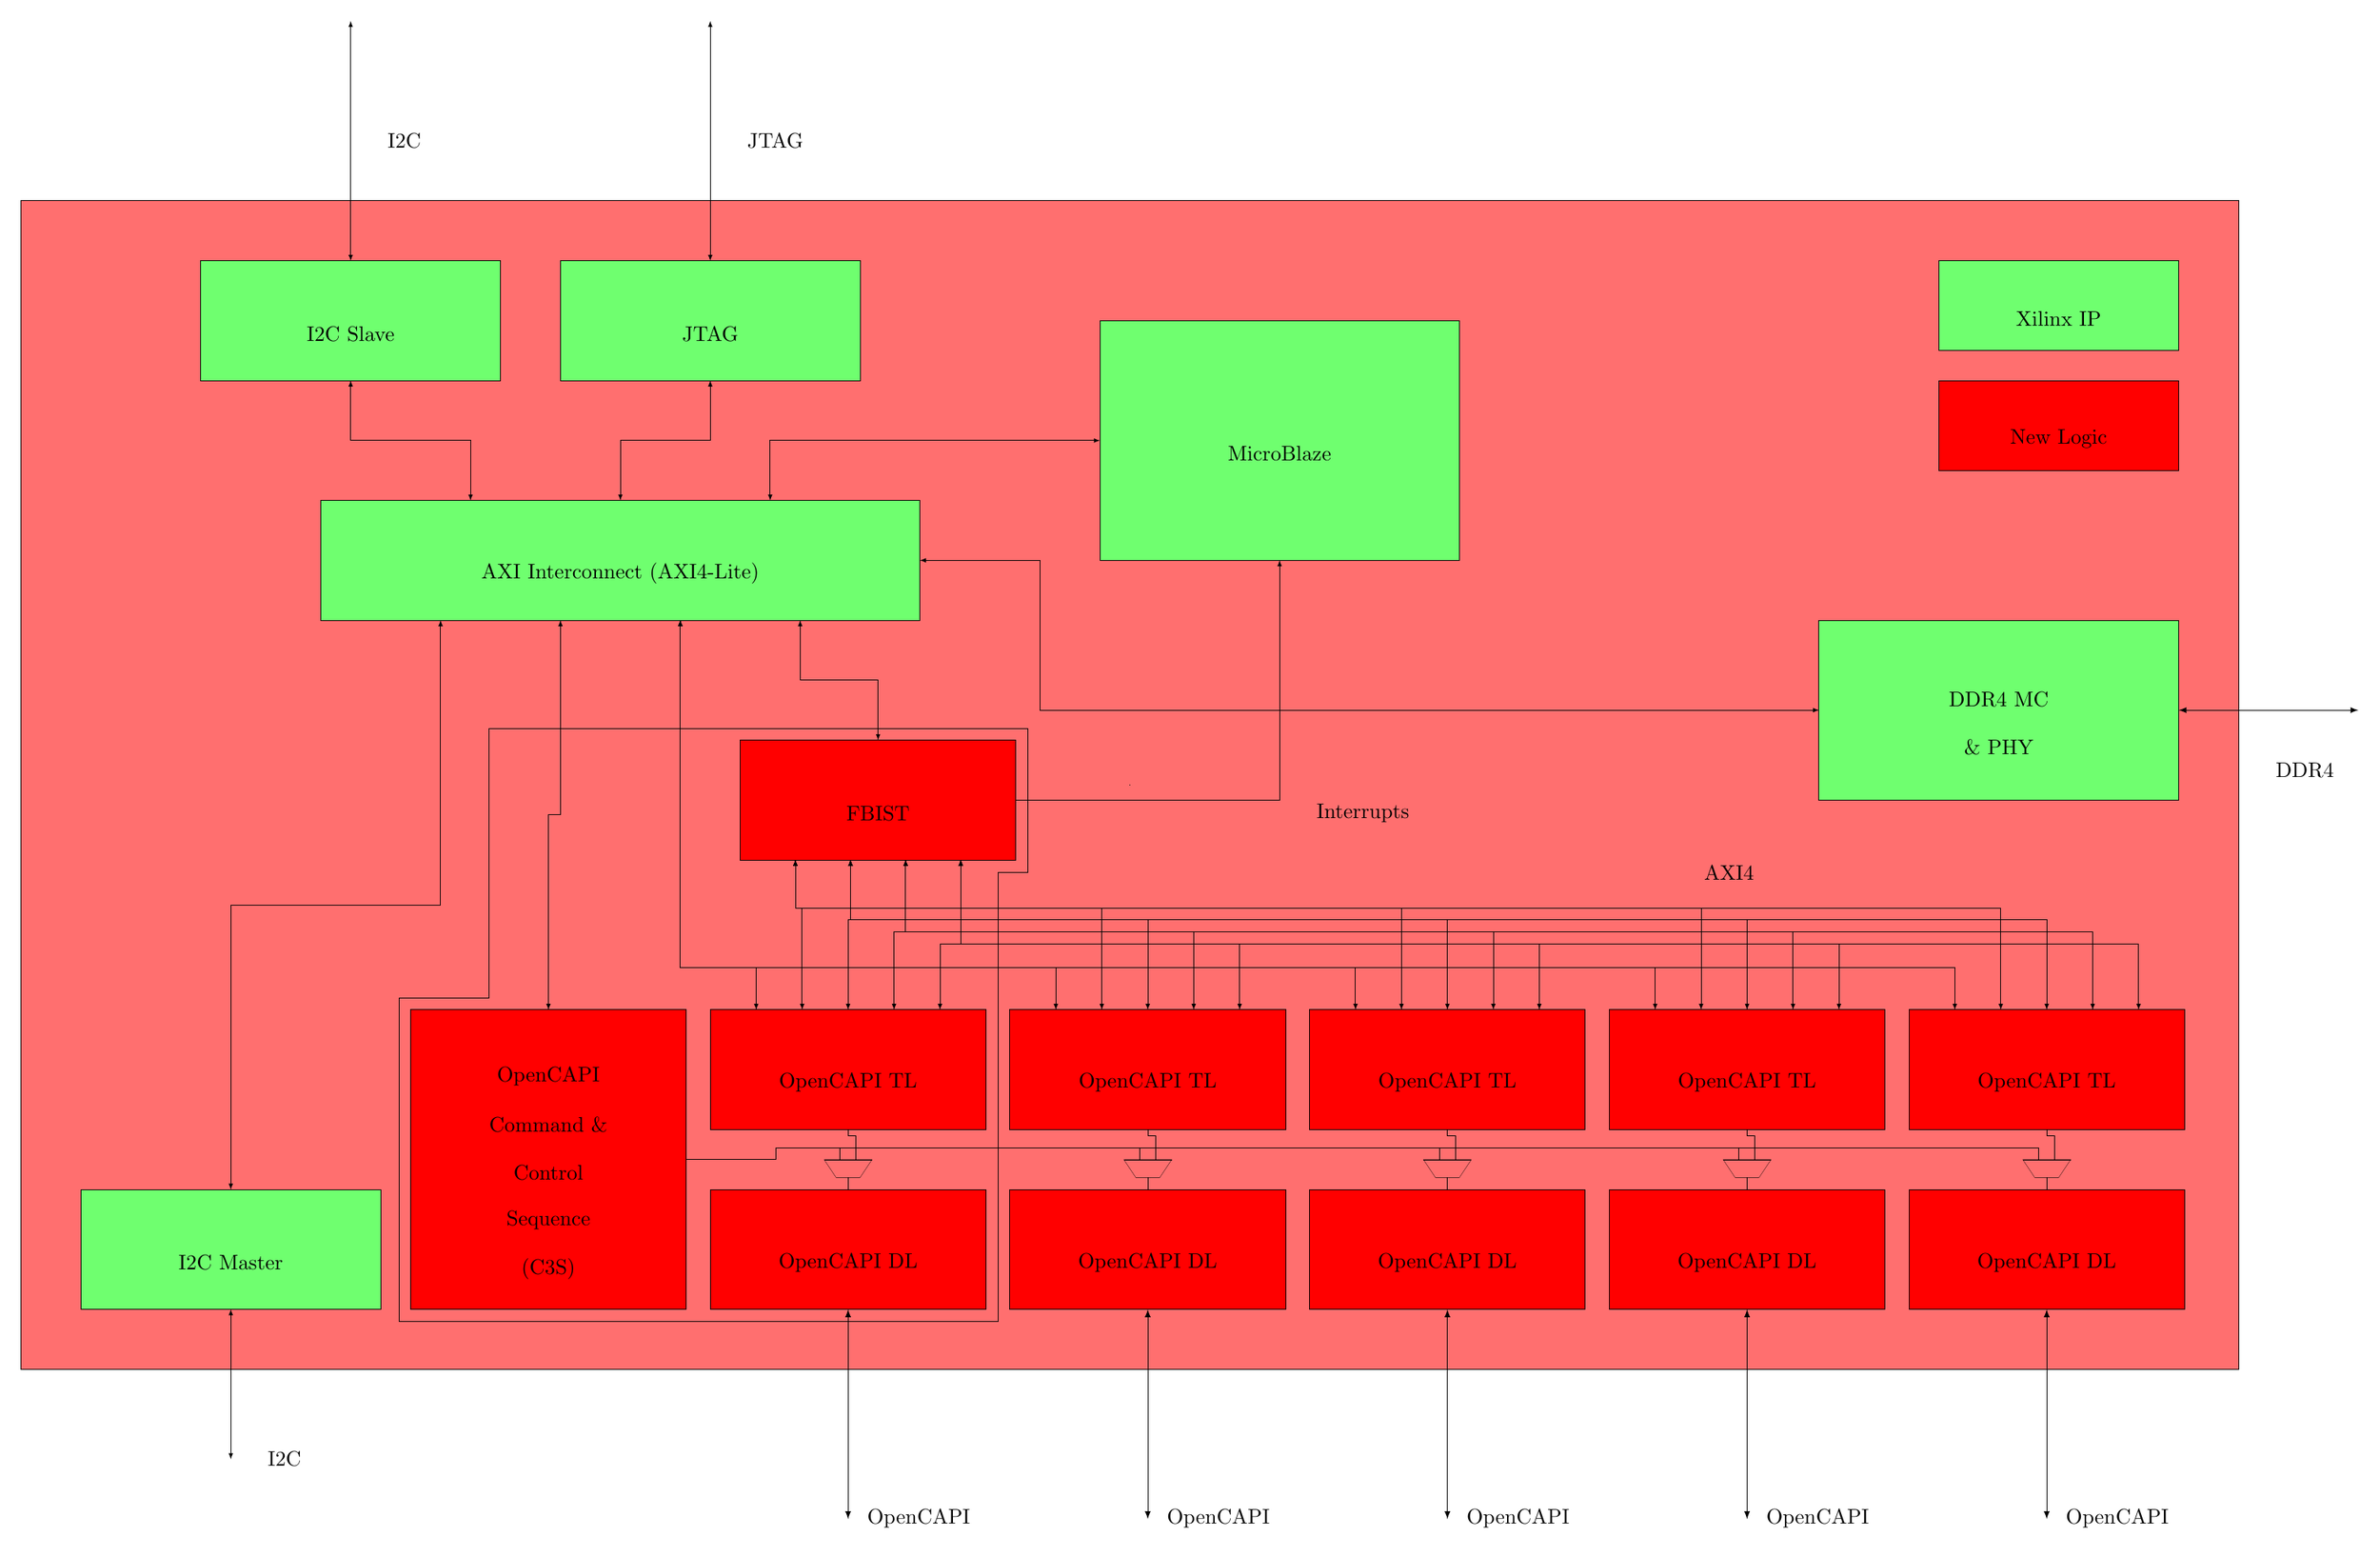
\begin{tikzpicture}
\pgftransformxscale{1.000000}
\pgftransformyscale{-1.000000}
\definecolor{dialinecolor}{rgb}{0.000000, 0.000000, 0.000000}
\pgfsetstrokecolor{dialinecolor}
\definecolor{dialinecolor}{rgb}{1.000000, 1.000000, 1.000000}
\pgfsetfillcolor{dialinecolor}
\pgfsetlinewidth{0.000000\du}
\pgfsetdash{}{0pt}
\pgfsetdash{}{0pt}
\pgfsetmiterjoin
\definecolor{dialinecolor}{rgb}{1.000000, 0.435294, 0.435294}
\pgfsetfillcolor{dialinecolor}
\fill (6.000000\du,-1.000000\du)--(6.000000\du,18.500000\du)--(43.000000\du,18.500000\du)--(43.000000\du,-1.000000\du)--cycle;
\definecolor{dialinecolor}{rgb}{0.000000, 0.000000, 0.000000}
\pgfsetstrokecolor{dialinecolor}
\draw (6.000000\du,-1.000000\du)--(6.000000\du,18.500000\du)--(43.000000\du,18.500000\du)--(43.000000\du,-1.000000\du)--cycle;
\pgfsetlinewidth{0.100000\du}
\pgfsetdash{{\pgflinewidth}{0.200000\du}}{0cm}
\pgfsetdash{{\pgflinewidth}{0.200000\du}}{0cm}
\pgfsetmiterjoin
\pgfsetbuttcap
\definecolor{dialinecolor}{rgb}{0.000000, 0.000000, 0.000000}
\pgfsetstrokecolor{dialinecolor}
\draw (13.800000\du,7.800000\du)--(22.800000\du,7.800000\du)--(22.800000\du,10.200000\du)--(22.300000\du,10.200000\du)--(22.300000\du,17.700000\du)--(12.300000\du,17.700000\du)--(12.300000\du,12.300000\du)--(13.800000\du,12.300000\du)--cycle;
\pgfsetlinewidth{0.000000\du}
\pgfsetdash{}{0pt}
\pgfsetdash{}{0pt}
\pgfsetmiterjoin
\definecolor{dialinecolor}{rgb}{0.435294, 1.000000, 0.435294}
\pgfsetfillcolor{dialinecolor}
\fill (7.000000\du,15.500000\du)--(7.000000\du,17.500000\du)--(12.000000\du,17.500000\du)--(12.000000\du,15.500000\du)--cycle;
\definecolor{dialinecolor}{rgb}{0.000000, 0.000000, 0.000000}
\pgfsetstrokecolor{dialinecolor}
\draw (7.000000\du,15.500000\du)--(7.000000\du,17.500000\du)--(12.000000\du,17.500000\du)--(12.000000\du,15.500000\du)--cycle;
% setfont left to latex
\definecolor{dialinecolor}{rgb}{0.000000, 0.000000, 0.000000}
\pgfsetstrokecolor{dialinecolor}
\node at (9.500000\du,16.721250\du){I2C Master};
\pgfsetlinewidth{0.000000\du}
\pgfsetdash{}{0pt}
\pgfsetdash{}{0pt}
\pgfsetmiterjoin
\definecolor{dialinecolor}{rgb}{0.435294, 1.000000, 0.435294}
\pgfsetfillcolor{dialinecolor}
\fill (15.000000\du,0.000000\du)--(15.000000\du,2.000000\du)--(20.000000\du,2.000000\du)--(20.000000\du,0.000000\du)--cycle;
\definecolor{dialinecolor}{rgb}{0.000000, 0.000000, 0.000000}
\pgfsetstrokecolor{dialinecolor}
\draw (15.000000\du,0.000000\du)--(15.000000\du,2.000000\du)--(20.000000\du,2.000000\du)--(20.000000\du,0.000000\du)--cycle;
% setfont left to latex
\definecolor{dialinecolor}{rgb}{0.000000, 0.000000, 0.000000}
\pgfsetstrokecolor{dialinecolor}
\node at (17.500000\du,1.221250\du){JTAG};
\pgfsetlinewidth{0.000000\du}
\pgfsetdash{}{0pt}
\pgfsetdash{}{0pt}
\pgfsetmiterjoin
\definecolor{dialinecolor}{rgb}{1.000000, 0.000000, 0.000000}
\pgfsetfillcolor{dialinecolor}
\fill (18.000000\du,8.000000\du)--(18.000000\du,10.000000\du)--(22.600000\du,10.000000\du)--(22.600000\du,8.000000\du)--cycle;
\definecolor{dialinecolor}{rgb}{0.000000, 0.000000, 0.000000}
\pgfsetstrokecolor{dialinecolor}
\draw (18.000000\du,8.000000\du)--(18.000000\du,10.000000\du)--(22.600000\du,10.000000\du)--(22.600000\du,8.000000\du)--cycle;
% setfont left to latex
\definecolor{dialinecolor}{rgb}{0.000000, 0.000000, 0.000000}
\pgfsetstrokecolor{dialinecolor}
\node at (20.300000\du,9.221250\du){FBIST};
\pgfsetlinewidth{0.000000\du}
\pgfsetdash{}{0pt}
\pgfsetdash{}{0pt}
\pgfsetmiterjoin
\pgfsetbuttcap
{
\definecolor{dialinecolor}{rgb}{0.000000, 0.000000, 0.000000}
\pgfsetfillcolor{dialinecolor}
% was here!!!
\pgfsetarrowsstart{latex}
\pgfsetarrowsend{latex}
{\pgfsetcornersarced{\pgfpoint{0.000000\du}{0.000000\du}}\definecolor{dialinecolor}{rgb}{0.000000, 0.000000, 0.000000}
\pgfsetstrokecolor{dialinecolor}
\draw (17.500000\du,2.000000\du)--(17.500000\du,3.000000\du)--(16.000000\du,3.000000\du)--(16.000000\du,4.000000\du);
}}
\pgfsetlinewidth{0.000000\du}
\pgfsetdash{}{0pt}
\pgfsetdash{}{0pt}
\pgfsetmiterjoin
\definecolor{dialinecolor}{rgb}{0.435294, 1.000000, 0.435294}
\pgfsetfillcolor{dialinecolor}
\fill (38.000000\du,0.000000\du)--(38.000000\du,1.500000\du)--(42.000000\du,1.500000\du)--(42.000000\du,0.000000\du)--cycle;
\definecolor{dialinecolor}{rgb}{0.000000, 0.000000, 0.000000}
\pgfsetstrokecolor{dialinecolor}
\draw (38.000000\du,0.000000\du)--(38.000000\du,1.500000\du)--(42.000000\du,1.500000\du)--(42.000000\du,0.000000\du)--cycle;
% setfont left to latex
\definecolor{dialinecolor}{rgb}{0.000000, 0.000000, 0.000000}
\pgfsetstrokecolor{dialinecolor}
\node at (40.000000\du,0.971250\du){Xilinx IP};
\pgfsetlinewidth{0.000000\du}
\pgfsetdash{}{0pt}
\pgfsetdash{}{0pt}
\pgfsetmiterjoin
\definecolor{dialinecolor}{rgb}{0.435294, 1.000000, 0.435294}
\pgfsetfillcolor{dialinecolor}
\fill (9.000000\du,0.000000\du)--(9.000000\du,2.000000\du)--(14.000000\du,2.000000\du)--(14.000000\du,0.000000\du)--cycle;
\definecolor{dialinecolor}{rgb}{0.000000, 0.000000, 0.000000}
\pgfsetstrokecolor{dialinecolor}
\draw (9.000000\du,0.000000\du)--(9.000000\du,2.000000\du)--(14.000000\du,2.000000\du)--(14.000000\du,0.000000\du)--cycle;
% setfont left to latex
\definecolor{dialinecolor}{rgb}{0.000000, 0.000000, 0.000000}
\pgfsetstrokecolor{dialinecolor}
\node at (11.500000\du,1.221250\du){I2C Slave};
\pgfsetlinewidth{0.000000\du}
\pgfsetdash{}{0pt}
\pgfsetdash{}{0pt}
\pgfsetmiterjoin
\pgfsetbuttcap
{
\definecolor{dialinecolor}{rgb}{0.000000, 0.000000, 0.000000}
\pgfsetfillcolor{dialinecolor}
% was here!!!
\pgfsetarrowsstart{latex}
\pgfsetarrowsend{latex}
{\pgfsetcornersarced{\pgfpoint{0.000000\du}{0.000000\du}}\definecolor{dialinecolor}{rgb}{0.000000, 0.000000, 0.000000}
\pgfsetstrokecolor{dialinecolor}
\draw (11.500000\du,2.000000\du)--(11.500000\du,3.000000\du)--(13.500000\du,3.000000\du)--(13.500000\du,4.000000\du);
}}
\pgfsetlinewidth{0.000000\du}
\pgfsetdash{}{0pt}
\pgfsetdash{}{0pt}
\pgfsetmiterjoin
\definecolor{dialinecolor}{rgb}{1.000000, 0.000000, 0.000000}
\pgfsetfillcolor{dialinecolor}
\fill (38.000000\du,2.000000\du)--(38.000000\du,3.500000\du)--(42.000000\du,3.500000\du)--(42.000000\du,2.000000\du)--cycle;
\definecolor{dialinecolor}{rgb}{0.000000, 0.000000, 0.000000}
\pgfsetstrokecolor{dialinecolor}
\draw (38.000000\du,2.000000\du)--(38.000000\du,3.500000\du)--(42.000000\du,3.500000\du)--(42.000000\du,2.000000\du)--cycle;
% setfont left to latex
\definecolor{dialinecolor}{rgb}{0.000000, 0.000000, 0.000000}
\pgfsetstrokecolor{dialinecolor}
\node at (40.000000\du,2.971250\du){New Logic};
% setfont left to latex
\definecolor{dialinecolor}{rgb}{0.000000, 0.000000, 0.000000}
\pgfsetstrokecolor{dialinecolor}
\node[anchor=west] at (12.000000\du,-2.000000\du){I2C};
\pgfsetlinewidth{0.000000\du}
\pgfsetdash{}{0pt}
\pgfsetdash{}{0pt}
\pgfsetmiterjoin
\definecolor{dialinecolor}{rgb}{1.000000, 0.000000, 0.000000}
\pgfsetfillcolor{dialinecolor}
\fill (12.500000\du,12.500000\du)--(12.500000\du,17.500000\du)--(17.100000\du,17.500000\du)--(17.100000\du,12.500000\du)--cycle;
\definecolor{dialinecolor}{rgb}{0.000000, 0.000000, 0.000000}
\pgfsetstrokecolor{dialinecolor}
\draw (12.500000\du,12.500000\du)--(12.500000\du,17.500000\du)--(17.100000\du,17.500000\du)--(17.100000\du,12.500000\du)--cycle;
% setfont left to latex
\definecolor{dialinecolor}{rgb}{0.000000, 0.000000, 0.000000}
\pgfsetstrokecolor{dialinecolor}
\node at (14.800000\du,13.621250\du){OpenCAPI};
% setfont left to latex
\definecolor{dialinecolor}{rgb}{0.000000, 0.000000, 0.000000}
\pgfsetstrokecolor{dialinecolor}
\node at (14.800000\du,14.421250\du){Command \&};
% setfont left to latex
\definecolor{dialinecolor}{rgb}{0.000000, 0.000000, 0.000000}
\pgfsetstrokecolor{dialinecolor}
\node at (14.800000\du,15.221250\du){Control};
% setfont left to latex
\definecolor{dialinecolor}{rgb}{0.000000, 0.000000, 0.000000}
\pgfsetstrokecolor{dialinecolor}
\node at (14.800000\du,16.021250\du){Sequence};
% setfont left to latex
\definecolor{dialinecolor}{rgb}{0.000000, 0.000000, 0.000000}
\pgfsetstrokecolor{dialinecolor}
\node at (14.800000\du,16.821250\du){(C3S)};
\pgfsetlinewidth{0.000000\du}
\pgfsetdash{}{0pt}
\pgfsetdash{}{0pt}
\pgfsetmiterjoin
\definecolor{dialinecolor}{rgb}{0.435294, 1.000000, 0.435294}
\pgfsetfillcolor{dialinecolor}
\fill (24.000000\du,1.000000\du)--(24.000000\du,5.000000\du)--(30.000000\du,5.000000\du)--(30.000000\du,1.000000\du)--cycle;
\definecolor{dialinecolor}{rgb}{0.000000, 0.000000, 0.000000}
\pgfsetstrokecolor{dialinecolor}
\draw (24.000000\du,1.000000\du)--(24.000000\du,5.000000\du)--(30.000000\du,5.000000\du)--(30.000000\du,1.000000\du)--cycle;
% setfont left to latex
\definecolor{dialinecolor}{rgb}{0.000000, 0.000000, 0.000000}
\pgfsetstrokecolor{dialinecolor}
\node at (27.000000\du,3.221250\du){MicroBlaze};
% setfont left to latex
\definecolor{dialinecolor}{rgb}{0.000000, 0.000000, 0.000000}
\pgfsetstrokecolor{dialinecolor}
\node[anchor=west] at (18.000000\du,-2.000000\du){JTAG};
\pgfsetlinewidth{0.000000\du}
\pgfsetdash{}{0pt}
\pgfsetdash{}{0pt}
\pgfsetmiterjoin
\definecolor{dialinecolor}{rgb}{0.435294, 1.000000, 0.435294}
\pgfsetfillcolor{dialinecolor}
\fill (11.000000\du,4.000000\du)--(11.000000\du,6.000000\du)--(21.000000\du,6.000000\du)--(21.000000\du,4.000000\du)--cycle;
\definecolor{dialinecolor}{rgb}{0.000000, 0.000000, 0.000000}
\pgfsetstrokecolor{dialinecolor}
\draw (11.000000\du,4.000000\du)--(11.000000\du,6.000000\du)--(21.000000\du,6.000000\du)--(21.000000\du,4.000000\du)--cycle;
% setfont left to latex
\definecolor{dialinecolor}{rgb}{0.000000, 0.000000, 0.000000}
\pgfsetstrokecolor{dialinecolor}
\node at (16.000000\du,5.221250\du){AXI Interconnect (AXI4-Lite)};
\pgfsetlinewidth{0.000000\du}
\pgfsetdash{}{0pt}
\pgfsetdash{}{0pt}
\pgfsetbuttcap
{
\definecolor{dialinecolor}{rgb}{0.000000, 0.000000, 0.000000}
\pgfsetfillcolor{dialinecolor}
% was here!!!
\definecolor{dialinecolor}{rgb}{0.000000, 0.000000, 0.000000}
\pgfsetstrokecolor{dialinecolor}
\draw (11.000000\du,4.000000\du)--(21.000000\du,4.000000\du);
}
\pgfsetlinewidth{0.000000\du}
\pgfsetdash{}{0pt}
\pgfsetdash{}{0pt}
\pgfsetmiterjoin
\pgfsetbuttcap
{
\definecolor{dialinecolor}{rgb}{0.000000, 0.000000, 0.000000}
\pgfsetfillcolor{dialinecolor}
% was here!!!
\pgfsetarrowsstart{latex}
\pgfsetarrowsend{latex}
{\pgfsetcornersarced{\pgfpoint{0.000000\du}{0.000000\du}}\definecolor{dialinecolor}{rgb}{0.000000, 0.000000, 0.000000}
\pgfsetstrokecolor{dialinecolor}
\draw (13.000000\du,6.000000\du)--(13.000000\du,10.749756\du)--(9.500000\du,10.749756\du)--(9.500000\du,15.499512\du);
}}
% setfont left to latex
\definecolor{dialinecolor}{rgb}{0.000000, 0.000000, 0.000000}
\pgfsetstrokecolor{dialinecolor}
\node[anchor=west] at (10.000000\du,20.000000\du){I2C};
% setfont left to latex
\definecolor{dialinecolor}{rgb}{0.000000, 0.000000, 0.000000}
\pgfsetstrokecolor{dialinecolor}
\node[anchor=west] at (27.500000\du,9.221250\du){Interrupts};
\pgfsetlinewidth{0.000000\du}
\pgfsetdash{}{0pt}
\pgfsetdash{}{0pt}
\pgfsetmiterjoin
\definecolor{dialinecolor}{rgb}{1.000000, 0.000000, 0.000000}
\pgfsetfillcolor{dialinecolor}
\fill (32.500000\du,15.500000\du)--(32.500000\du,17.500000\du)--(37.100000\du,17.500000\du)--(37.100000\du,15.500000\du)--cycle;
\definecolor{dialinecolor}{rgb}{0.000000, 0.000000, 0.000000}
\pgfsetstrokecolor{dialinecolor}
\draw (32.500000\du,15.500000\du)--(32.500000\du,17.500000\du)--(37.100000\du,17.500000\du)--(37.100000\du,15.500000\du)--cycle;
% setfont left to latex
\definecolor{dialinecolor}{rgb}{0.000000, 0.000000, 0.000000}
\pgfsetstrokecolor{dialinecolor}
\node at (34.800000\du,16.721250\du){OpenCAPI DL};
\pgfsetlinewidth{0.300000\du}
\pgfsetdash{}{0pt}
\pgfsetdash{}{0pt}
\pgfsetbuttcap
{
\definecolor{dialinecolor}{rgb}{0.000000, 0.000000, 0.000000}
\pgfsetfillcolor{dialinecolor}
% was here!!!
\pgfsetarrowsstart{latex}
\pgfsetarrowsend{latex}
\definecolor{dialinecolor}{rgb}{0.000000, 0.000000, 0.000000}
\pgfsetstrokecolor{dialinecolor}
\draw (34.800000\du,17.500000\du)--(34.800000\du,21.000000\du);
}
% setfont left to latex
\definecolor{dialinecolor}{rgb}{0.000000, 0.000000, 0.000000}
\pgfsetstrokecolor{dialinecolor}
\node[anchor=west] at (35.000000\du,21.000000\du){OpenCAPI};
\pgfsetlinewidth{0.000000\du}
\pgfsetdash{}{0pt}
\pgfsetdash{}{0pt}
\pgfsetmiterjoin
\definecolor{dialinecolor}{rgb}{1.000000, 0.000000, 0.000000}
\pgfsetfillcolor{dialinecolor}
\fill (27.500000\du,15.500000\du)--(27.500000\du,17.500000\du)--(32.100000\du,17.500000\du)--(32.100000\du,15.500000\du)--cycle;
\definecolor{dialinecolor}{rgb}{0.000000, 0.000000, 0.000000}
\pgfsetstrokecolor{dialinecolor}
\draw (27.500000\du,15.500000\du)--(27.500000\du,17.500000\du)--(32.100000\du,17.500000\du)--(32.100000\du,15.500000\du)--cycle;
% setfont left to latex
\definecolor{dialinecolor}{rgb}{0.000000, 0.000000, 0.000000}
\pgfsetstrokecolor{dialinecolor}
\node at (29.800000\du,16.721250\du){OpenCAPI DL};
\pgfsetlinewidth{0.300000\du}
\pgfsetdash{}{0pt}
\pgfsetdash{}{0pt}
\pgfsetbuttcap
{
\definecolor{dialinecolor}{rgb}{0.000000, 0.000000, 0.000000}
\pgfsetfillcolor{dialinecolor}
% was here!!!
\pgfsetarrowsstart{latex}
\pgfsetarrowsend{latex}
\definecolor{dialinecolor}{rgb}{0.000000, 0.000000, 0.000000}
\pgfsetstrokecolor{dialinecolor}
\draw (29.800000\du,17.500000\du)--(29.800000\du,21.000000\du);
}
% setfont left to latex
\definecolor{dialinecolor}{rgb}{0.000000, 0.000000, 0.000000}
\pgfsetstrokecolor{dialinecolor}
\node[anchor=west] at (30.000000\du,21.000000\du){OpenCAPI};
\pgfsetlinewidth{0.000000\du}
\pgfsetdash{}{0pt}
\pgfsetdash{}{0pt}
\pgfsetmiterjoin
\definecolor{dialinecolor}{rgb}{1.000000, 0.000000, 0.000000}
\pgfsetfillcolor{dialinecolor}
\fill (37.500000\du,15.500000\du)--(37.500000\du,17.500000\du)--(42.100000\du,17.500000\du)--(42.100000\du,15.500000\du)--cycle;
\definecolor{dialinecolor}{rgb}{0.000000, 0.000000, 0.000000}
\pgfsetstrokecolor{dialinecolor}
\draw (37.500000\du,15.500000\du)--(37.500000\du,17.500000\du)--(42.100000\du,17.500000\du)--(42.100000\du,15.500000\du)--cycle;
% setfont left to latex
\definecolor{dialinecolor}{rgb}{0.000000, 0.000000, 0.000000}
\pgfsetstrokecolor{dialinecolor}
\node at (39.800000\du,16.721250\du){OpenCAPI DL};
\pgfsetlinewidth{0.300000\du}
\pgfsetdash{}{0pt}
\pgfsetdash{}{0pt}
\pgfsetbuttcap
{
\definecolor{dialinecolor}{rgb}{0.000000, 0.000000, 0.000000}
\pgfsetfillcolor{dialinecolor}
% was here!!!
\pgfsetarrowsstart{latex}
\pgfsetarrowsend{latex}
\definecolor{dialinecolor}{rgb}{0.000000, 0.000000, 0.000000}
\pgfsetstrokecolor{dialinecolor}
\draw (39.800000\du,17.500000\du)--(39.800000\du,21.000000\du);
}
% setfont left to latex
\definecolor{dialinecolor}{rgb}{0.000000, 0.000000, 0.000000}
\pgfsetstrokecolor{dialinecolor}
\node[anchor=west] at (40.000000\du,21.000000\du){OpenCAPI};
\pgfsetlinewidth{0.000000\du}
\pgfsetdash{}{0pt}
\pgfsetdash{}{0pt}
\pgfsetmiterjoin
\definecolor{dialinecolor}{rgb}{1.000000, 0.000000, 0.000000}
\pgfsetfillcolor{dialinecolor}
\fill (22.500000\du,15.500000\du)--(22.500000\du,17.500000\du)--(27.100000\du,17.500000\du)--(27.100000\du,15.500000\du)--cycle;
\definecolor{dialinecolor}{rgb}{0.000000, 0.000000, 0.000000}
\pgfsetstrokecolor{dialinecolor}
\draw (22.500000\du,15.500000\du)--(22.500000\du,17.500000\du)--(27.100000\du,17.500000\du)--(27.100000\du,15.500000\du)--cycle;
% setfont left to latex
\definecolor{dialinecolor}{rgb}{0.000000, 0.000000, 0.000000}
\pgfsetstrokecolor{dialinecolor}
\node at (24.800000\du,16.721250\du){OpenCAPI DL};
\pgfsetlinewidth{0.300000\du}
\pgfsetdash{}{0pt}
\pgfsetdash{}{0pt}
\pgfsetbuttcap
{
\definecolor{dialinecolor}{rgb}{0.000000, 0.000000, 0.000000}
\pgfsetfillcolor{dialinecolor}
% was here!!!
\pgfsetarrowsstart{latex}
\pgfsetarrowsend{latex}
\definecolor{dialinecolor}{rgb}{0.000000, 0.000000, 0.000000}
\pgfsetstrokecolor{dialinecolor}
\draw (24.800000\du,17.500000\du)--(24.800000\du,21.000000\du);
}
% setfont left to latex
\definecolor{dialinecolor}{rgb}{0.000000, 0.000000, 0.000000}
\pgfsetstrokecolor{dialinecolor}
\node[anchor=west] at (25.000000\du,21.000000\du){OpenCAPI};
\pgfsetlinewidth{0.000000\du}
\pgfsetdash{}{0pt}
\pgfsetdash{}{0pt}
\pgfsetmiterjoin
\definecolor{dialinecolor}{rgb}{1.000000, 0.000000, 0.000000}
\pgfsetfillcolor{dialinecolor}
\fill (17.500000\du,15.500000\du)--(17.500000\du,17.500000\du)--(22.100000\du,17.500000\du)--(22.100000\du,15.500000\du)--cycle;
\definecolor{dialinecolor}{rgb}{0.000000, 0.000000, 0.000000}
\pgfsetstrokecolor{dialinecolor}
\draw (17.500000\du,15.500000\du)--(17.500000\du,17.500000\du)--(22.100000\du,17.500000\du)--(22.100000\du,15.500000\du)--cycle;
% setfont left to latex
\definecolor{dialinecolor}{rgb}{0.000000, 0.000000, 0.000000}
\pgfsetstrokecolor{dialinecolor}
\node at (19.800000\du,16.721250\du){OpenCAPI DL};
\pgfsetlinewidth{0.300000\du}
\pgfsetdash{}{0pt}
\pgfsetdash{}{0pt}
\pgfsetbuttcap
{
\definecolor{dialinecolor}{rgb}{0.000000, 0.000000, 0.000000}
\pgfsetfillcolor{dialinecolor}
% was here!!!
\pgfsetarrowsstart{latex}
\pgfsetarrowsend{latex}
\definecolor{dialinecolor}{rgb}{0.000000, 0.000000, 0.000000}
\pgfsetstrokecolor{dialinecolor}
\draw (19.800000\du,17.500000\du)--(19.800000\du,21.000000\du);
}
% setfont left to latex
\definecolor{dialinecolor}{rgb}{0.000000, 0.000000, 0.000000}
\pgfsetstrokecolor{dialinecolor}
\node[anchor=west] at (20.000000\du,21.000000\du){OpenCAPI};
\pgfsetlinewidth{0.000000\du}
\pgfsetdash{}{0pt}
\pgfsetdash{}{0pt}
\pgfsetmiterjoin
\definecolor{dialinecolor}{rgb}{1.000000, 0.000000, 0.000000}
\pgfsetfillcolor{dialinecolor}
\fill (17.500000\du,12.500000\du)--(17.500000\du,14.500000\du)--(22.100000\du,14.500000\du)--(22.100000\du,12.500000\du)--cycle;
\definecolor{dialinecolor}{rgb}{0.000000, 0.000000, 0.000000}
\pgfsetstrokecolor{dialinecolor}
\draw (17.500000\du,12.500000\du)--(17.500000\du,14.500000\du)--(22.100000\du,14.500000\du)--(22.100000\du,12.500000\du)--cycle;
% setfont left to latex
\definecolor{dialinecolor}{rgb}{0.000000, 0.000000, 0.000000}
\pgfsetstrokecolor{dialinecolor}
\node at (19.800000\du,13.721250\du){OpenCAPI TL};
\pgfsetlinewidth{0.000000\du}
\pgfsetdash{}{0pt}
\pgfsetdash{}{0pt}
\pgfsetmiterjoin
\definecolor{dialinecolor}{rgb}{1.000000, 0.000000, 0.000000}
\pgfsetfillcolor{dialinecolor}
\fill (22.500000\du,12.500000\du)--(22.500000\du,14.500000\du)--(27.100000\du,14.500000\du)--(27.100000\du,12.500000\du)--cycle;
\definecolor{dialinecolor}{rgb}{0.000000, 0.000000, 0.000000}
\pgfsetstrokecolor{dialinecolor}
\draw (22.500000\du,12.500000\du)--(22.500000\du,14.500000\du)--(27.100000\du,14.500000\du)--(27.100000\du,12.500000\du)--cycle;
% setfont left to latex
\definecolor{dialinecolor}{rgb}{0.000000, 0.000000, 0.000000}
\pgfsetstrokecolor{dialinecolor}
\node at (24.800000\du,13.721250\du){OpenCAPI TL};
\pgfsetlinewidth{0.000000\du}
\pgfsetdash{}{0pt}
\pgfsetdash{}{0pt}
\pgfsetmiterjoin
\definecolor{dialinecolor}{rgb}{1.000000, 0.000000, 0.000000}
\pgfsetfillcolor{dialinecolor}
\fill (27.500000\du,12.500000\du)--(27.500000\du,14.500000\du)--(32.100000\du,14.500000\du)--(32.100000\du,12.500000\du)--cycle;
\definecolor{dialinecolor}{rgb}{0.000000, 0.000000, 0.000000}
\pgfsetstrokecolor{dialinecolor}
\draw (27.500000\du,12.500000\du)--(27.500000\du,14.500000\du)--(32.100000\du,14.500000\du)--(32.100000\du,12.500000\du)--cycle;
% setfont left to latex
\definecolor{dialinecolor}{rgb}{0.000000, 0.000000, 0.000000}
\pgfsetstrokecolor{dialinecolor}
\node at (29.800000\du,13.721250\du){OpenCAPI TL};
\pgfsetlinewidth{0.000000\du}
\pgfsetdash{}{0pt}
\pgfsetdash{}{0pt}
\pgfsetmiterjoin
\definecolor{dialinecolor}{rgb}{1.000000, 0.000000, 0.000000}
\pgfsetfillcolor{dialinecolor}
\fill (32.500000\du,12.500000\du)--(32.500000\du,14.500000\du)--(37.100000\du,14.500000\du)--(37.100000\du,12.500000\du)--cycle;
\definecolor{dialinecolor}{rgb}{0.000000, 0.000000, 0.000000}
\pgfsetstrokecolor{dialinecolor}
\draw (32.500000\du,12.500000\du)--(32.500000\du,14.500000\du)--(37.100000\du,14.500000\du)--(37.100000\du,12.500000\du)--cycle;
% setfont left to latex
\definecolor{dialinecolor}{rgb}{0.000000, 0.000000, 0.000000}
\pgfsetstrokecolor{dialinecolor}
\node at (34.800000\du,13.721250\du){OpenCAPI TL};
\pgfsetlinewidth{0.000000\du}
\pgfsetdash{}{0pt}
\pgfsetdash{}{0pt}
\pgfsetmiterjoin
\definecolor{dialinecolor}{rgb}{1.000000, 0.000000, 0.000000}
\pgfsetfillcolor{dialinecolor}
\fill (37.500000\du,12.500000\du)--(37.500000\du,14.500000\du)--(42.100000\du,14.500000\du)--(42.100000\du,12.500000\du)--cycle;
\definecolor{dialinecolor}{rgb}{0.000000, 0.000000, 0.000000}
\pgfsetstrokecolor{dialinecolor}
\draw (37.500000\du,12.500000\du)--(37.500000\du,14.500000\du)--(42.100000\du,14.500000\du)--(42.100000\du,12.500000\du)--cycle;
% setfont left to latex
\definecolor{dialinecolor}{rgb}{0.000000, 0.000000, 0.000000}
\pgfsetstrokecolor{dialinecolor}
\node at (39.800000\du,13.721250\du){OpenCAPI TL};
\pgfsetlinewidth{0.000000\du}
\pgfsetdash{}{0pt}
\pgfsetdash{}{0pt}
\pgfsetbuttcap
{
\definecolor{dialinecolor}{rgb}{0.000000, 0.000000, 0.000000}
\pgfsetfillcolor{dialinecolor}
% was here!!!
\definecolor{dialinecolor}{rgb}{0.000000, 0.000000, 0.000000}
\pgfsetstrokecolor{dialinecolor}
\draw (19.800000\du,15.300000\du)--(19.800000\du,15.500000\du);
}
\pgfsetlinewidth{0.100000\du}
\pgfsetdash{}{0pt}
\pgfsetdash{}{0pt}
\pgfsetmiterjoin
\pgfsetbuttcap
\definecolor{dialinecolor}{rgb}{0.000000, 0.000000, 0.000000}
\pgfsetstrokecolor{dialinecolor}
\draw (19.400000\du,15.000000\du)--(20.200000\du,15.000000\du)--(20.000000\du,15.300000\du)--(19.600000\du,15.300000\du)--cycle;
\pgfsetlinewidth{0.100000\du}
\pgfsetdash{}{0pt}
\pgfsetdash{}{0pt}
\pgfsetbuttcap
{
\definecolor{dialinecolor}{rgb}{0.000000, 0.000000, 0.000000}
\pgfsetfillcolor{dialinecolor}
% was here!!!
\definecolor{dialinecolor}{rgb}{0.000000, 0.000000, 0.000000}
\pgfsetstrokecolor{dialinecolor}
\draw (19.400000\du,15.000000\du)--(20.200000\du,15.000000\du);
}
\pgfsetlinewidth{0.000000\du}
\pgfsetdash{}{0pt}
\pgfsetdash{}{0pt}
\pgfsetbuttcap
{
\definecolor{dialinecolor}{rgb}{0.000000, 0.000000, 0.000000}
\pgfsetfillcolor{dialinecolor}
% was here!!!
\definecolor{dialinecolor}{rgb}{0.000000, 0.000000, 0.000000}
\pgfsetstrokecolor{dialinecolor}
\draw (24.800000\du,15.300000\du)--(24.800000\du,15.500000\du);
}
\pgfsetlinewidth{0.100000\du}
\pgfsetdash{}{0pt}
\pgfsetdash{}{0pt}
\pgfsetmiterjoin
\pgfsetbuttcap
\definecolor{dialinecolor}{rgb}{0.000000, 0.000000, 0.000000}
\pgfsetstrokecolor{dialinecolor}
\draw (24.400000\du,15.000000\du)--(25.200000\du,15.000000\du)--(25.000000\du,15.300000\du)--(24.600000\du,15.300000\du)--cycle;
\pgfsetlinewidth{0.100000\du}
\pgfsetdash{}{0pt}
\pgfsetdash{}{0pt}
\pgfsetbuttcap
{
\definecolor{dialinecolor}{rgb}{0.000000, 0.000000, 0.000000}
\pgfsetfillcolor{dialinecolor}
% was here!!!
\definecolor{dialinecolor}{rgb}{0.000000, 0.000000, 0.000000}
\pgfsetstrokecolor{dialinecolor}
\draw (24.400000\du,15.000000\du)--(25.200000\du,15.000000\du);
}
\pgfsetlinewidth{0.000000\du}
\pgfsetdash{}{0pt}
\pgfsetdash{}{0pt}
\pgfsetbuttcap
{
\definecolor{dialinecolor}{rgb}{0.000000, 0.000000, 0.000000}
\pgfsetfillcolor{dialinecolor}
% was here!!!
\definecolor{dialinecolor}{rgb}{0.000000, 0.000000, 0.000000}
\pgfsetstrokecolor{dialinecolor}
\draw (29.800000\du,15.300000\du)--(29.800000\du,15.500000\du);
}
\pgfsetlinewidth{0.100000\du}
\pgfsetdash{}{0pt}
\pgfsetdash{}{0pt}
\pgfsetmiterjoin
\pgfsetbuttcap
\definecolor{dialinecolor}{rgb}{0.000000, 0.000000, 0.000000}
\pgfsetstrokecolor{dialinecolor}
\draw (29.400000\du,15.000000\du)--(30.200000\du,15.000000\du)--(30.000000\du,15.300000\du)--(29.600000\du,15.300000\du)--cycle;
\pgfsetlinewidth{0.100000\du}
\pgfsetdash{}{0pt}
\pgfsetdash{}{0pt}
\pgfsetbuttcap
{
\definecolor{dialinecolor}{rgb}{0.000000, 0.000000, 0.000000}
\pgfsetfillcolor{dialinecolor}
% was here!!!
\definecolor{dialinecolor}{rgb}{0.000000, 0.000000, 0.000000}
\pgfsetstrokecolor{dialinecolor}
\draw (29.400000\du,15.000000\du)--(30.200000\du,15.000000\du);
}
\pgfsetlinewidth{0.000000\du}
\pgfsetdash{}{0pt}
\pgfsetdash{}{0pt}
\pgfsetbuttcap
{
\definecolor{dialinecolor}{rgb}{0.000000, 0.000000, 0.000000}
\pgfsetfillcolor{dialinecolor}
% was here!!!
\definecolor{dialinecolor}{rgb}{0.000000, 0.000000, 0.000000}
\pgfsetstrokecolor{dialinecolor}
\draw (34.800000\du,15.300000\du)--(34.800000\du,15.500000\du);
}
\pgfsetlinewidth{0.100000\du}
\pgfsetdash{}{0pt}
\pgfsetdash{}{0pt}
\pgfsetmiterjoin
\pgfsetbuttcap
\definecolor{dialinecolor}{rgb}{0.000000, 0.000000, 0.000000}
\pgfsetstrokecolor{dialinecolor}
\draw (34.400000\du,15.000000\du)--(35.200000\du,15.000000\du)--(35.000000\du,15.300000\du)--(34.600000\du,15.300000\du)--cycle;
\pgfsetlinewidth{0.100000\du}
\pgfsetdash{}{0pt}
\pgfsetdash{}{0pt}
\pgfsetbuttcap
{
\definecolor{dialinecolor}{rgb}{0.000000, 0.000000, 0.000000}
\pgfsetfillcolor{dialinecolor}
% was here!!!
\definecolor{dialinecolor}{rgb}{0.000000, 0.000000, 0.000000}
\pgfsetstrokecolor{dialinecolor}
\draw (34.400000\du,15.000000\du)--(35.200000\du,15.000000\du);
}
\pgfsetlinewidth{0.000000\du}
\pgfsetdash{}{0pt}
\pgfsetdash{}{0pt}
\pgfsetbuttcap
{
\definecolor{dialinecolor}{rgb}{0.000000, 0.000000, 0.000000}
\pgfsetfillcolor{dialinecolor}
% was here!!!
\definecolor{dialinecolor}{rgb}{0.000000, 0.000000, 0.000000}
\pgfsetstrokecolor{dialinecolor}
\draw (39.800000\du,15.300000\du)--(39.800000\du,15.500000\du);
}
\pgfsetlinewidth{0.100000\du}
\pgfsetdash{}{0pt}
\pgfsetdash{}{0pt}
\pgfsetmiterjoin
\pgfsetbuttcap
\definecolor{dialinecolor}{rgb}{0.000000, 0.000000, 0.000000}
\pgfsetstrokecolor{dialinecolor}
\draw (39.400000\du,15.000000\du)--(40.200000\du,15.000000\du)--(40.000000\du,15.300000\du)--(39.600000\du,15.300000\du)--cycle;
\pgfsetlinewidth{0.100000\du}
\pgfsetdash{}{0pt}
\pgfsetdash{}{0pt}
\pgfsetbuttcap
{
\definecolor{dialinecolor}{rgb}{0.000000, 0.000000, 0.000000}
\pgfsetfillcolor{dialinecolor}
% was here!!!
\definecolor{dialinecolor}{rgb}{0.000000, 0.000000, 0.000000}
\pgfsetstrokecolor{dialinecolor}
\draw (39.400000\du,15.000000\du)--(40.200000\du,15.000000\du);
}
\pgfsetlinewidth{0.000000\du}
\pgfsetdash{}{0pt}
\pgfsetdash{}{0pt}
\pgfsetmiterjoin
\pgfsetbuttcap
{
\definecolor{dialinecolor}{rgb}{0.000000, 0.000000, 0.000000}
\pgfsetfillcolor{dialinecolor}
% was here!!!
{\pgfsetcornersarced{\pgfpoint{0.000000\du}{0.000000\du}}\definecolor{dialinecolor}{rgb}{0.000000, 0.000000, 0.000000}
\pgfsetstrokecolor{dialinecolor}
\draw (19.800000\du,14.500000\du)--(19.800000\du,14.600000\du)--(19.933300\du,14.600000\du)--(19.933300\du,15.000000\du);
}}
\pgfsetlinewidth{0.000000\du}
\pgfsetdash{}{0pt}
\pgfsetdash{}{0pt}
\pgfsetmiterjoin
\pgfsetbuttcap
{
\definecolor{dialinecolor}{rgb}{0.000000, 0.000000, 0.000000}
\pgfsetfillcolor{dialinecolor}
% was here!!!
{\pgfsetcornersarced{\pgfpoint{0.000000\du}{0.000000\du}}\definecolor{dialinecolor}{rgb}{0.000000, 0.000000, 0.000000}
\pgfsetstrokecolor{dialinecolor}
\draw (24.800000\du,14.500000\du)--(24.800000\du,14.600000\du)--(24.933300\du,14.600000\du)--(24.933300\du,15.000000\du);
}}
\pgfsetlinewidth{0.000000\du}
\pgfsetdash{}{0pt}
\pgfsetdash{}{0pt}
\pgfsetmiterjoin
\pgfsetbuttcap
{
\definecolor{dialinecolor}{rgb}{0.000000, 0.000000, 0.000000}
\pgfsetfillcolor{dialinecolor}
% was here!!!
{\pgfsetcornersarced{\pgfpoint{0.000000\du}{0.000000\du}}\definecolor{dialinecolor}{rgb}{0.000000, 0.000000, 0.000000}
\pgfsetstrokecolor{dialinecolor}
\draw (29.800000\du,14.500000\du)--(29.800000\du,14.600000\du)--(29.933300\du,14.600000\du)--(29.933300\du,15.000000\du);
}}
\pgfsetlinewidth{0.000000\du}
\pgfsetdash{}{0pt}
\pgfsetdash{}{0pt}
\pgfsetmiterjoin
\pgfsetbuttcap
{
\definecolor{dialinecolor}{rgb}{0.000000, 0.000000, 0.000000}
\pgfsetfillcolor{dialinecolor}
% was here!!!
{\pgfsetcornersarced{\pgfpoint{0.000000\du}{0.000000\du}}\definecolor{dialinecolor}{rgb}{0.000000, 0.000000, 0.000000}
\pgfsetstrokecolor{dialinecolor}
\draw (34.800000\du,14.500000\du)--(34.800000\du,14.600000\du)--(34.933300\du,14.600000\du)--(34.933300\du,15.000000\du);
}}
\pgfsetlinewidth{0.000000\du}
\pgfsetdash{}{0pt}
\pgfsetdash{}{0pt}
\pgfsetmiterjoin
\pgfsetbuttcap
{
\definecolor{dialinecolor}{rgb}{0.000000, 0.000000, 0.000000}
\pgfsetfillcolor{dialinecolor}
% was here!!!
{\pgfsetcornersarced{\pgfpoint{0.000000\du}{0.000000\du}}\definecolor{dialinecolor}{rgb}{0.000000, 0.000000, 0.000000}
\pgfsetstrokecolor{dialinecolor}
\draw (39.800000\du,14.500000\du)--(39.800000\du,14.600000\du)--(39.933300\du,14.600000\du)--(39.933300\du,15.000000\du);
}}
\pgfsetlinewidth{0.000000\du}
\pgfsetdash{}{0pt}
\pgfsetdash{}{0pt}
\pgfsetmiterjoin
\pgfsetbuttcap
{
\definecolor{dialinecolor}{rgb}{0.000000, 0.000000, 0.000000}
\pgfsetfillcolor{dialinecolor}
% was here!!!
{\pgfsetcornersarced{\pgfpoint{0.000000\du}{0.000000\du}}\definecolor{dialinecolor}{rgb}{0.000000, 0.000000, 0.000000}
\pgfsetstrokecolor{dialinecolor}
\draw (17.100000\du,15.000000\du)--(18.600000\du,15.000000\du)--(18.600000\du,14.800000\du)--(19.666700\du,14.800000\du)--(19.666700\du,15.000000\du);
}}
\pgfsetlinewidth{0.000000\du}
\pgfsetdash{}{0pt}
\pgfsetdash{}{0pt}
\pgfsetmiterjoin
\pgfsetbuttcap
{
\definecolor{dialinecolor}{rgb}{0.000000, 0.000000, 0.000000}
\pgfsetfillcolor{dialinecolor}
% was here!!!
{\pgfsetcornersarced{\pgfpoint{0.000000\du}{0.000000\du}}\definecolor{dialinecolor}{rgb}{0.000000, 0.000000, 0.000000}
\pgfsetstrokecolor{dialinecolor}
\draw (19.666700\du,15.000000\du)--(19.666700\du,14.800000\du)--(24.666700\du,14.800000\du)--(24.666700\du,15.000000\du);
}}
\pgfsetlinewidth{0.000000\du}
\pgfsetdash{}{0pt}
\pgfsetdash{}{0pt}
\pgfsetmiterjoin
\pgfsetbuttcap
{
\definecolor{dialinecolor}{rgb}{0.000000, 0.000000, 0.000000}
\pgfsetfillcolor{dialinecolor}
% was here!!!
{\pgfsetcornersarced{\pgfpoint{0.000000\du}{0.000000\du}}\definecolor{dialinecolor}{rgb}{0.000000, 0.000000, 0.000000}
\pgfsetstrokecolor{dialinecolor}
\draw (24.666700\du,15.000000\du)--(24.666700\du,14.800000\du)--(29.666700\du,14.800000\du)--(29.666700\du,15.000000\du);
}}
\pgfsetlinewidth{0.000000\du}
\pgfsetdash{}{0pt}
\pgfsetdash{}{0pt}
\pgfsetmiterjoin
\pgfsetbuttcap
{
\definecolor{dialinecolor}{rgb}{0.000000, 0.000000, 0.000000}
\pgfsetfillcolor{dialinecolor}
% was here!!!
{\pgfsetcornersarced{\pgfpoint{0.000000\du}{0.000000\du}}\definecolor{dialinecolor}{rgb}{0.000000, 0.000000, 0.000000}
\pgfsetstrokecolor{dialinecolor}
\draw (29.666700\du,15.000000\du)--(29.666700\du,14.800000\du)--(34.666700\du,14.800000\du)--(34.666700\du,15.000000\du);
}}
\pgfsetlinewidth{0.000000\du}
\pgfsetdash{}{0pt}
\pgfsetdash{}{0pt}
\pgfsetmiterjoin
\pgfsetbuttcap
{
\definecolor{dialinecolor}{rgb}{0.000000, 0.000000, 0.000000}
\pgfsetfillcolor{dialinecolor}
% was here!!!
{\pgfsetcornersarced{\pgfpoint{0.000000\du}{0.000000\du}}\definecolor{dialinecolor}{rgb}{0.000000, 0.000000, 0.000000}
\pgfsetstrokecolor{dialinecolor}
\draw (34.666700\du,15.000000\du)--(34.666700\du,14.800000\du)--(39.666700\du,14.800000\du)--(39.666700\du,15.000000\du);
}}
\pgfsetlinewidth{0.000000\du}
\pgfsetdash{}{0pt}
\pgfsetdash{}{0pt}
\pgfsetbuttcap
{
\definecolor{dialinecolor}{rgb}{0.000000, 0.000000, 0.000000}
\pgfsetfillcolor{dialinecolor}
% was here!!!
\definecolor{dialinecolor}{rgb}{0.000000, 0.000000, 0.000000}
\pgfsetstrokecolor{dialinecolor}
\draw (18.000000\du,10.000000\du)--(22.600000\du,10.000000\du);
}
\pgfsetlinewidth{0.000000\du}
\pgfsetdash{}{0pt}
\pgfsetdash{}{0pt}
\pgfsetbuttcap
{
\definecolor{dialinecolor}{rgb}{0.000000, 0.000000, 0.000000}
\pgfsetfillcolor{dialinecolor}
% was here!!!
\definecolor{dialinecolor}{rgb}{0.000000, 0.000000, 0.000000}
\pgfsetstrokecolor{dialinecolor}
\draw (17.500000\du,12.500000\du)--(22.100000\du,12.500000\du);
}
\pgfsetlinewidth{0.000000\du}
\pgfsetdash{}{0pt}
\pgfsetdash{}{0pt}
\pgfsetbuttcap
{
\definecolor{dialinecolor}{rgb}{0.000000, 0.000000, 0.000000}
\pgfsetfillcolor{dialinecolor}
% was here!!!
\definecolor{dialinecolor}{rgb}{0.000000, 0.000000, 0.000000}
\pgfsetstrokecolor{dialinecolor}
\draw (22.500000\du,12.500000\du)--(27.100000\du,12.500000\du);
}
\pgfsetlinewidth{0.000000\du}
\pgfsetdash{}{0pt}
\pgfsetdash{}{0pt}
\pgfsetbuttcap
{
\definecolor{dialinecolor}{rgb}{0.000000, 0.000000, 0.000000}
\pgfsetfillcolor{dialinecolor}
% was here!!!
\definecolor{dialinecolor}{rgb}{0.000000, 0.000000, 0.000000}
\pgfsetstrokecolor{dialinecolor}
\draw (27.500000\du,12.500000\du)--(32.100000\du,12.500000\du);
}
\pgfsetlinewidth{0.000000\du}
\pgfsetdash{}{0pt}
\pgfsetdash{}{0pt}
\pgfsetbuttcap
{
\definecolor{dialinecolor}{rgb}{0.000000, 0.000000, 0.000000}
\pgfsetfillcolor{dialinecolor}
% was here!!!
\definecolor{dialinecolor}{rgb}{0.000000, 0.000000, 0.000000}
\pgfsetstrokecolor{dialinecolor}
\draw (32.500000\du,12.500000\du)--(37.100000\du,12.500000\du);
}
\pgfsetlinewidth{0.000000\du}
\pgfsetdash{}{0pt}
\pgfsetdash{}{0pt}
\pgfsetbuttcap
{
\definecolor{dialinecolor}{rgb}{0.000000, 0.000000, 0.000000}
\pgfsetfillcolor{dialinecolor}
% was here!!!
\definecolor{dialinecolor}{rgb}{0.000000, 0.000000, 0.000000}
\pgfsetstrokecolor{dialinecolor}
\draw (37.500000\du,12.500000\du)--(42.100000\du,12.500000\du);
}
\pgfsetlinewidth{0.000000\du}
\pgfsetdash{}{0pt}
\pgfsetdash{}{0pt}
\pgfsetmiterjoin
\pgfsetbuttcap
{
\definecolor{dialinecolor}{rgb}{0.000000, 0.000000, 0.000000}
\pgfsetfillcolor{dialinecolor}
% was here!!!
\pgfsetarrowsstart{latex}
\pgfsetarrowsend{latex}
{\pgfsetcornersarced{\pgfpoint{0.000000\du}{0.000000\du}}\definecolor{dialinecolor}{rgb}{0.000000, 0.000000, 0.000000}
\pgfsetstrokecolor{dialinecolor}
\draw (18.920000\du,10.000000\du)--(18.920000\du,10.800000\du)--(19.033300\du,10.800000\du)--(19.033300\du,12.500000\du);
}}
\pgfsetlinewidth{0.000000\du}
\pgfsetdash{}{0pt}
\pgfsetdash{}{0pt}
\pgfsetmiterjoin
\pgfsetbuttcap
{
\definecolor{dialinecolor}{rgb}{0.000000, 0.000000, 0.000000}
\pgfsetfillcolor{dialinecolor}
% was here!!!
\pgfsetarrowsstart{latex}
\pgfsetarrowsend{latex}
{\pgfsetcornersarced{\pgfpoint{0.000000\du}{0.000000\du}}\definecolor{dialinecolor}{rgb}{0.000000, 0.000000, 0.000000}
\pgfsetstrokecolor{dialinecolor}
\draw (19.840000\du,10.000000\du)--(19.840000\du,11.000000\du)--(19.800000\du,11.000000\du)--(19.800000\du,12.500000\du);
}}
\pgfsetlinewidth{0.000000\du}
\pgfsetdash{}{0pt}
\pgfsetdash{}{0pt}
\pgfsetmiterjoin
\pgfsetbuttcap
{
\definecolor{dialinecolor}{rgb}{0.000000, 0.000000, 0.000000}
\pgfsetfillcolor{dialinecolor}
% was here!!!
\pgfsetarrowsstart{latex}
\pgfsetarrowsend{latex}
{\pgfsetcornersarced{\pgfpoint{0.000000\du}{0.000000\du}}\definecolor{dialinecolor}{rgb}{0.000000, 0.000000, 0.000000}
\pgfsetstrokecolor{dialinecolor}
\draw (20.760000\du,10.000000\du)--(20.760000\du,11.200000\du)--(20.566700\du,11.200000\du)--(20.566700\du,12.500000\du);
}}
\pgfsetlinewidth{0.000000\du}
\pgfsetdash{}{0pt}
\pgfsetdash{}{0pt}
\pgfsetmiterjoin
\pgfsetbuttcap
{
\definecolor{dialinecolor}{rgb}{0.000000, 0.000000, 0.000000}
\pgfsetfillcolor{dialinecolor}
% was here!!!
\pgfsetarrowsstart{latex}
\pgfsetarrowsend{latex}
{\pgfsetcornersarced{\pgfpoint{0.000000\du}{0.000000\du}}\definecolor{dialinecolor}{rgb}{0.000000, 0.000000, 0.000000}
\pgfsetstrokecolor{dialinecolor}
\draw (21.680000\du,10.000000\du)--(21.680000\du,11.400000\du)--(21.333300\du,11.400000\du)--(21.333300\du,12.500000\du);
}}
\pgfsetlinewidth{0.000000\du}
\pgfsetdash{}{0pt}
\pgfsetdash{}{0pt}
\pgfsetmiterjoin
\pgfsetbuttcap
{
\definecolor{dialinecolor}{rgb}{0.000000, 0.000000, 0.000000}
\pgfsetfillcolor{dialinecolor}
% was here!!!
\pgfsetarrowsstart{latex}
\pgfsetarrowsend{latex}
{\pgfsetcornersarced{\pgfpoint{0.000000\du}{0.000000\du}}\definecolor{dialinecolor}{rgb}{0.000000, 0.000000, 0.000000}
\pgfsetstrokecolor{dialinecolor}
\draw (18.920000\du,10.000000\du)--(18.920000\du,10.800000\du)--(24.033300\du,10.800000\du)--(24.033300\du,12.500000\du);
}}
\pgfsetlinewidth{0.000000\du}
\pgfsetdash{}{0pt}
\pgfsetdash{}{0pt}
\pgfsetmiterjoin
\pgfsetbuttcap
{
\definecolor{dialinecolor}{rgb}{0.000000, 0.000000, 0.000000}
\pgfsetfillcolor{dialinecolor}
% was here!!!
\pgfsetarrowsstart{latex}
\pgfsetarrowsend{latex}
{\pgfsetcornersarced{\pgfpoint{0.000000\du}{0.000000\du}}\definecolor{dialinecolor}{rgb}{0.000000, 0.000000, 0.000000}
\pgfsetstrokecolor{dialinecolor}
\draw (19.840000\du,10.000000\du)--(19.840000\du,11.000000\du)--(24.800000\du,11.000000\du)--(24.800000\du,12.500000\du);
}}
\pgfsetlinewidth{0.000000\du}
\pgfsetdash{}{0pt}
\pgfsetdash{}{0pt}
\pgfsetmiterjoin
\pgfsetbuttcap
{
\definecolor{dialinecolor}{rgb}{0.000000, 0.000000, 0.000000}
\pgfsetfillcolor{dialinecolor}
% was here!!!
\pgfsetarrowsstart{latex}
\pgfsetarrowsend{latex}
{\pgfsetcornersarced{\pgfpoint{0.000000\du}{0.000000\du}}\definecolor{dialinecolor}{rgb}{0.000000, 0.000000, 0.000000}
\pgfsetstrokecolor{dialinecolor}
\draw (20.760000\du,10.000000\du)--(20.760000\du,11.200000\du)--(25.566700\du,11.200000\du)--(25.566700\du,12.500000\du);
}}
\pgfsetlinewidth{0.000000\du}
\pgfsetdash{}{0pt}
\pgfsetdash{}{0pt}
\pgfsetmiterjoin
\pgfsetbuttcap
{
\definecolor{dialinecolor}{rgb}{0.000000, 0.000000, 0.000000}
\pgfsetfillcolor{dialinecolor}
% was here!!!
\pgfsetarrowsstart{latex}
\pgfsetarrowsend{latex}
{\pgfsetcornersarced{\pgfpoint{0.000000\du}{0.000000\du}}\definecolor{dialinecolor}{rgb}{0.000000, 0.000000, 0.000000}
\pgfsetstrokecolor{dialinecolor}
\draw (21.680000\du,10.000000\du)--(21.680000\du,11.400000\du)--(26.333300\du,11.400000\du)--(26.333300\du,12.500000\du);
}}
\pgfsetlinewidth{0.000000\du}
\pgfsetdash{}{0pt}
\pgfsetdash{}{0pt}
\pgfsetmiterjoin
\pgfsetbuttcap
{
\definecolor{dialinecolor}{rgb}{0.000000, 0.000000, 0.000000}
\pgfsetfillcolor{dialinecolor}
% was here!!!
\pgfsetarrowsstart{latex}
\pgfsetarrowsend{latex}
{\pgfsetcornersarced{\pgfpoint{0.000000\du}{0.000000\du}}\definecolor{dialinecolor}{rgb}{0.000000, 0.000000, 0.000000}
\pgfsetstrokecolor{dialinecolor}
\draw (18.920000\du,10.000000\du)--(18.920000\du,10.800000\du)--(29.033300\du,10.800000\du)--(29.033300\du,12.500000\du);
}}
\pgfsetlinewidth{0.000000\du}
\pgfsetdash{}{0pt}
\pgfsetdash{}{0pt}
\pgfsetmiterjoin
\pgfsetbuttcap
{
\definecolor{dialinecolor}{rgb}{0.000000, 0.000000, 0.000000}
\pgfsetfillcolor{dialinecolor}
% was here!!!
\pgfsetarrowsstart{latex}
\pgfsetarrowsend{latex}
{\pgfsetcornersarced{\pgfpoint{0.000000\du}{0.000000\du}}\definecolor{dialinecolor}{rgb}{0.000000, 0.000000, 0.000000}
\pgfsetstrokecolor{dialinecolor}
\draw (19.840000\du,10.000000\du)--(19.840000\du,11.000000\du)--(29.800000\du,11.000000\du)--(29.800000\du,12.500000\du);
}}
\pgfsetlinewidth{0.000000\du}
\pgfsetdash{}{0pt}
\pgfsetdash{}{0pt}
\pgfsetmiterjoin
\pgfsetbuttcap
{
\definecolor{dialinecolor}{rgb}{0.000000, 0.000000, 0.000000}
\pgfsetfillcolor{dialinecolor}
% was here!!!
\pgfsetarrowsstart{latex}
\pgfsetarrowsend{latex}
{\pgfsetcornersarced{\pgfpoint{0.000000\du}{0.000000\du}}\definecolor{dialinecolor}{rgb}{0.000000, 0.000000, 0.000000}
\pgfsetstrokecolor{dialinecolor}
\draw (20.760000\du,10.000000\du)--(20.760000\du,11.200000\du)--(30.566700\du,11.200000\du)--(30.566700\du,12.500000\du);
}}
\pgfsetlinewidth{0.000000\du}
\pgfsetdash{}{0pt}
\pgfsetdash{}{0pt}
\pgfsetmiterjoin
\pgfsetbuttcap
{
\definecolor{dialinecolor}{rgb}{0.000000, 0.000000, 0.000000}
\pgfsetfillcolor{dialinecolor}
% was here!!!
\pgfsetarrowsstart{latex}
\pgfsetarrowsend{latex}
{\pgfsetcornersarced{\pgfpoint{0.000000\du}{0.000000\du}}\definecolor{dialinecolor}{rgb}{0.000000, 0.000000, 0.000000}
\pgfsetstrokecolor{dialinecolor}
\draw (21.680000\du,10.000000\du)--(21.680000\du,11.400000\du)--(31.333300\du,11.400000\du)--(31.333300\du,12.500000\du);
}}
\pgfsetlinewidth{0.000000\du}
\pgfsetdash{}{0pt}
\pgfsetdash{}{0pt}
\pgfsetmiterjoin
\pgfsetbuttcap
{
\definecolor{dialinecolor}{rgb}{0.000000, 0.000000, 0.000000}
\pgfsetfillcolor{dialinecolor}
% was here!!!
\pgfsetarrowsstart{latex}
\pgfsetarrowsend{latex}
{\pgfsetcornersarced{\pgfpoint{0.000000\du}{0.000000\du}}\definecolor{dialinecolor}{rgb}{0.000000, 0.000000, 0.000000}
\pgfsetstrokecolor{dialinecolor}
\draw (18.920000\du,10.000000\du)--(18.920000\du,10.800000\du)--(34.033300\du,10.800000\du)--(34.033300\du,12.500000\du);
}}
\pgfsetlinewidth{0.000000\du}
\pgfsetdash{}{0pt}
\pgfsetdash{}{0pt}
\pgfsetmiterjoin
\pgfsetbuttcap
{
\definecolor{dialinecolor}{rgb}{0.000000, 0.000000, 0.000000}
\pgfsetfillcolor{dialinecolor}
% was here!!!
\pgfsetarrowsstart{latex}
\pgfsetarrowsend{latex}
{\pgfsetcornersarced{\pgfpoint{0.000000\du}{0.000000\du}}\definecolor{dialinecolor}{rgb}{0.000000, 0.000000, 0.000000}
\pgfsetstrokecolor{dialinecolor}
\draw (19.840000\du,10.000000\du)--(19.840000\du,11.000000\du)--(34.800000\du,11.000000\du)--(34.800000\du,12.500000\du);
}}
\pgfsetlinewidth{0.000000\du}
\pgfsetdash{}{0pt}
\pgfsetdash{}{0pt}
\pgfsetmiterjoin
\pgfsetbuttcap
{
\definecolor{dialinecolor}{rgb}{0.000000, 0.000000, 0.000000}
\pgfsetfillcolor{dialinecolor}
% was here!!!
\pgfsetarrowsstart{latex}
\pgfsetarrowsend{latex}
{\pgfsetcornersarced{\pgfpoint{0.000000\du}{0.000000\du}}\definecolor{dialinecolor}{rgb}{0.000000, 0.000000, 0.000000}
\pgfsetstrokecolor{dialinecolor}
\draw (20.760000\du,10.000000\du)--(20.760000\du,11.200000\du)--(35.566700\du,11.200000\du)--(35.566700\du,12.500000\du);
}}
\pgfsetlinewidth{0.000000\du}
\pgfsetdash{}{0pt}
\pgfsetdash{}{0pt}
\pgfsetmiterjoin
\pgfsetbuttcap
{
\definecolor{dialinecolor}{rgb}{0.000000, 0.000000, 0.000000}
\pgfsetfillcolor{dialinecolor}
% was here!!!
\pgfsetarrowsstart{latex}
\pgfsetarrowsend{latex}
{\pgfsetcornersarced{\pgfpoint{0.000000\du}{0.000000\du}}\definecolor{dialinecolor}{rgb}{0.000000, 0.000000, 0.000000}
\pgfsetstrokecolor{dialinecolor}
\draw (18.920000\du,10.000000\du)--(18.920000\du,10.800000\du)--(39.033300\du,10.800000\du)--(39.033300\du,12.500000\du);
}}
\pgfsetlinewidth{0.000000\du}
\pgfsetdash{}{0pt}
\pgfsetdash{}{0pt}
\pgfsetmiterjoin
\pgfsetbuttcap
{
\definecolor{dialinecolor}{rgb}{0.000000, 0.000000, 0.000000}
\pgfsetfillcolor{dialinecolor}
% was here!!!
\pgfsetarrowsstart{latex}
\pgfsetarrowsend{latex}
{\pgfsetcornersarced{\pgfpoint{0.000000\du}{0.000000\du}}\definecolor{dialinecolor}{rgb}{0.000000, 0.000000, 0.000000}
\pgfsetstrokecolor{dialinecolor}
\draw (19.840000\du,10.000000\du)--(19.840000\du,11.000000\du)--(39.800000\du,11.000000\du)--(39.800000\du,12.500000\du);
}}
\pgfsetlinewidth{0.000000\du}
\pgfsetdash{}{0pt}
\pgfsetdash{}{0pt}
\pgfsetmiterjoin
\pgfsetbuttcap
{
\definecolor{dialinecolor}{rgb}{0.000000, 0.000000, 0.000000}
\pgfsetfillcolor{dialinecolor}
% was here!!!
\pgfsetarrowsstart{latex}
\pgfsetarrowsend{latex}
{\pgfsetcornersarced{\pgfpoint{0.000000\du}{0.000000\du}}\definecolor{dialinecolor}{rgb}{0.000000, 0.000000, 0.000000}
\pgfsetstrokecolor{dialinecolor}
\draw (20.760000\du,10.000000\du)--(20.760000\du,11.200000\du)--(40.566700\du,11.200000\du)--(40.566700\du,12.500000\du);
}}
\pgfsetlinewidth{0.000000\du}
\pgfsetdash{}{0pt}
\pgfsetdash{}{0pt}
\pgfsetmiterjoin
\pgfsetbuttcap
{
\definecolor{dialinecolor}{rgb}{0.000000, 0.000000, 0.000000}
\pgfsetfillcolor{dialinecolor}
% was here!!!
\pgfsetarrowsstart{latex}
\pgfsetarrowsend{latex}
{\pgfsetcornersarced{\pgfpoint{0.000000\du}{0.000000\du}}\definecolor{dialinecolor}{rgb}{0.000000, 0.000000, 0.000000}
\pgfsetstrokecolor{dialinecolor}
\draw (21.680000\du,10.000000\du)--(21.680000\du,11.400000\du)--(41.333300\du,11.400000\du)--(41.333300\du,12.500000\du);
}}
\pgfsetlinewidth{0.000000\du}
\pgfsetdash{}{0pt}
\pgfsetdash{}{0pt}
\pgfsetmiterjoin
\pgfsetbuttcap
{
\definecolor{dialinecolor}{rgb}{0.000000, 0.000000, 0.000000}
\pgfsetfillcolor{dialinecolor}
% was here!!!
\pgfsetarrowsstart{latex}
\pgfsetarrowsend{latex}
{\pgfsetcornersarced{\pgfpoint{0.000000\du}{0.000000\du}}\definecolor{dialinecolor}{rgb}{0.000000, 0.000000, 0.000000}
\pgfsetstrokecolor{dialinecolor}
\draw (21.680000\du,10.000000\du)--(21.680000\du,11.400000\du)--(36.333300\du,11.400000\du)--(36.333300\du,12.500000\du);
}}
% setfont left to latex
\definecolor{dialinecolor}{rgb}{0.000000, 0.000000, 0.000000}
\pgfsetstrokecolor{dialinecolor}
\node at (34.500000\du,10.221250\du){AXI4};
\pgfsetlinewidth{0.000000\du}
\pgfsetdash{}{0pt}
\pgfsetdash{}{0pt}
\pgfsetbuttcap
{
\definecolor{dialinecolor}{rgb}{0.000000, 0.000000, 0.000000}
\pgfsetfillcolor{dialinecolor}
% was here!!!
\definecolor{dialinecolor}{rgb}{0.000000, 0.000000, 0.000000}
\pgfsetstrokecolor{dialinecolor}
\draw (11.000000\du,6.000000\du)--(21.000000\du,6.000000\du);
}
\pgfsetlinewidth{0.000000\du}
\pgfsetdash{}{0pt}
\pgfsetdash{}{0pt}
\pgfsetmiterjoin
\pgfsetbuttcap
{
\definecolor{dialinecolor}{rgb}{0.000000, 0.000000, 0.000000}
\pgfsetfillcolor{dialinecolor}
% was here!!!
\pgfsetarrowsstart{latex}
\pgfsetarrowsend{latex}
{\pgfsetcornersarced{\pgfpoint{0.000000\du}{0.000000\du}}\definecolor{dialinecolor}{rgb}{0.000000, 0.000000, 0.000000}
\pgfsetstrokecolor{dialinecolor}
\draw (19.000000\du,6.000000\du)--(19.000000\du,7.000000\du)--(20.300000\du,7.000000\du)--(20.300000\du,8.000000\du);
}}
\pgfsetlinewidth{0.000000\du}
\pgfsetdash{}{0pt}
\pgfsetdash{}{0pt}
\pgfsetmiterjoin
\pgfsetbuttcap
{
\definecolor{dialinecolor}{rgb}{0.000000, 0.000000, 0.000000}
\pgfsetfillcolor{dialinecolor}
% was here!!!
\pgfsetarrowsend{latex}
{\pgfsetcornersarced{\pgfpoint{0.000000\du}{0.000000\du}}\definecolor{dialinecolor}{rgb}{0.000000, 0.000000, 0.000000}
\pgfsetstrokecolor{dialinecolor}
\draw (22.600000\du,9.000000\du)--(27.000000\du,9.000000\du)--(27.000000\du,5.000000\du);
}}
\pgfsetlinewidth{0.000000\du}
\pgfsetdash{}{0pt}
\pgfsetdash{}{0pt}
\pgfsetmiterjoin
\pgfsetbuttcap
{
\definecolor{dialinecolor}{rgb}{0.000000, 0.000000, 0.000000}
\pgfsetfillcolor{dialinecolor}
% was here!!!
\pgfsetarrowsstart{latex}
\pgfsetarrowsend{latex}
{\pgfsetcornersarced{\pgfpoint{0.000000\du}{0.000000\du}}\definecolor{dialinecolor}{rgb}{0.000000, 0.000000, 0.000000}
\pgfsetstrokecolor{dialinecolor}
\draw (17.000000\du,6.000000\du)--(17.000000\du,11.800000\du)--(18.266700\du,11.800000\du)--(18.266700\du,12.500000\du);
}}
\pgfsetlinewidth{0.000000\du}
\pgfsetdash{}{0pt}
\pgfsetdash{}{0pt}
\pgfsetmiterjoin
\pgfsetbuttcap
{
\definecolor{dialinecolor}{rgb}{0.000000, 0.000000, 0.000000}
\pgfsetfillcolor{dialinecolor}
% was here!!!
\pgfsetarrowsstart{latex}
\pgfsetarrowsend{latex}
{\pgfsetcornersarced{\pgfpoint{0.000000\du}{0.000000\du}}\definecolor{dialinecolor}{rgb}{0.000000, 0.000000, 0.000000}
\pgfsetstrokecolor{dialinecolor}
\draw (17.000000\du,6.000000\du)--(17.000000\du,11.800000\du)--(23.266700\du,11.800000\du)--(23.266700\du,12.500000\du);
}}
\pgfsetlinewidth{0.000000\du}
\pgfsetdash{}{0pt}
\pgfsetdash{}{0pt}
\pgfsetmiterjoin
\pgfsetbuttcap
{
\definecolor{dialinecolor}{rgb}{0.000000, 0.000000, 0.000000}
\pgfsetfillcolor{dialinecolor}
% was here!!!
\pgfsetarrowsstart{latex}
\pgfsetarrowsend{latex}
{\pgfsetcornersarced{\pgfpoint{0.000000\du}{0.000000\du}}\definecolor{dialinecolor}{rgb}{0.000000, 0.000000, 0.000000}
\pgfsetstrokecolor{dialinecolor}
\draw (17.000000\du,6.000000\du)--(17.000000\du,11.800000\du)--(28.266700\du,11.800000\du)--(28.266700\du,12.500000\du);
}}
\pgfsetlinewidth{0.000000\du}
\pgfsetdash{}{0pt}
\pgfsetdash{}{0pt}
\pgfsetmiterjoin
\pgfsetbuttcap
{
\definecolor{dialinecolor}{rgb}{0.000000, 0.000000, 0.000000}
\pgfsetfillcolor{dialinecolor}
% was here!!!
\pgfsetarrowsstart{latex}
\pgfsetarrowsend{latex}
{\pgfsetcornersarced{\pgfpoint{0.000000\du}{0.000000\du}}\definecolor{dialinecolor}{rgb}{0.000000, 0.000000, 0.000000}
\pgfsetstrokecolor{dialinecolor}
\draw (17.000000\du,6.000000\du)--(17.000000\du,11.800000\du)--(33.266700\du,11.800000\du)--(33.266700\du,12.500000\du);
}}
\pgfsetlinewidth{0.000000\du}
\pgfsetdash{}{0pt}
\pgfsetdash{}{0pt}
\pgfsetmiterjoin
\pgfsetbuttcap
{
\definecolor{dialinecolor}{rgb}{0.000000, 0.000000, 0.000000}
\pgfsetfillcolor{dialinecolor}
% was here!!!
\pgfsetarrowsstart{latex}
\pgfsetarrowsend{latex}
{\pgfsetcornersarced{\pgfpoint{0.000000\du}{0.000000\du}}\definecolor{dialinecolor}{rgb}{0.000000, 0.000000, 0.000000}
\pgfsetstrokecolor{dialinecolor}
\draw (38.266700\du,12.500000\du)--(38.266700\du,11.800000\du)--(17.000000\du,11.800000\du)--(17.000000\du,6.000000\du);
}}
\pgfsetlinewidth{0.000000\du}
\pgfsetdash{}{0pt}
\pgfsetdash{}{0pt}
\pgfsetmiterjoin
\pgfsetbuttcap
{
\definecolor{dialinecolor}{rgb}{0.000000, 0.000000, 0.000000}
\pgfsetfillcolor{dialinecolor}
% was here!!!
\pgfsetarrowsstart{latex}
\pgfsetarrowsend{latex}
{\pgfsetcornersarced{\pgfpoint{0.000000\du}{0.000000\du}}\definecolor{dialinecolor}{rgb}{0.000000, 0.000000, 0.000000}
\pgfsetstrokecolor{dialinecolor}
\draw (14.800000\du,12.500000\du)--(14.800000\du,9.250000\du)--(15.000000\du,9.250000\du)--(15.000000\du,6.000000\du);
}}
\pgfsetlinewidth{0.000000\du}
\pgfsetdash{}{0pt}
\pgfsetdash{}{0pt}
\pgfsetbuttcap
{
\definecolor{dialinecolor}{rgb}{0.000000, 0.000000, 0.000000}
\pgfsetfillcolor{dialinecolor}
% was here!!!
\definecolor{dialinecolor}{rgb}{0.000000, 0.000000, 0.000000}
\pgfsetstrokecolor{dialinecolor}
\draw (24.500000\du,8.750000\du)--(24.500000\du,8.750000\du);
}
\pgfsetlinewidth{0.000000\du}
\pgfsetdash{}{0pt}
\pgfsetdash{}{0pt}
\pgfsetbuttcap
{
\definecolor{dialinecolor}{rgb}{0.000000, 0.000000, 0.000000}
\pgfsetfillcolor{dialinecolor}
% was here!!!
\pgfsetarrowsstart{latex}
\pgfsetarrowsend{latex}
\definecolor{dialinecolor}{rgb}{0.000000, 0.000000, 0.000000}
\pgfsetstrokecolor{dialinecolor}
\draw (9.500000\du,17.500000\du)--(9.500000\du,20.000000\du);
}
\pgfsetlinewidth{0.000000\du}
\pgfsetdash{}{0pt}
\pgfsetdash{}{0pt}
\pgfsetbuttcap
{
\definecolor{dialinecolor}{rgb}{0.000000, 0.000000, 0.000000}
\pgfsetfillcolor{dialinecolor}
% was here!!!
\pgfsetarrowsstart{latex}
\pgfsetarrowsend{latex}
\definecolor{dialinecolor}{rgb}{0.000000, 0.000000, 0.000000}
\pgfsetstrokecolor{dialinecolor}
\draw (11.500000\du,-4.000000\du)--(11.500000\du,0.000000\du);
}
\pgfsetlinewidth{0.000000\du}
\pgfsetdash{}{0pt}
\pgfsetdash{}{0pt}
\pgfsetbuttcap
{
\definecolor{dialinecolor}{rgb}{0.000000, 0.000000, 0.000000}
\pgfsetfillcolor{dialinecolor}
% was here!!!
\pgfsetarrowsstart{latex}
\pgfsetarrowsend{latex}
\definecolor{dialinecolor}{rgb}{0.000000, 0.000000, 0.000000}
\pgfsetstrokecolor{dialinecolor}
\draw (17.500000\du,-4.000000\du)--(17.500000\du,0.000000\du);
}
\pgfsetlinewidth{0.000000\du}
\pgfsetdash{}{0pt}
\pgfsetdash{}{0pt}
\pgfsetmiterjoin
\pgfsetbuttcap
{
\definecolor{dialinecolor}{rgb}{0.000000, 0.000000, 0.000000}
\pgfsetfillcolor{dialinecolor}
% was here!!!
\pgfsetarrowsstart{latex}
\pgfsetarrowsend{latex}
{\pgfsetcornersarced{\pgfpoint{0.000000\du}{0.000000\du}}\definecolor{dialinecolor}{rgb}{0.000000, 0.000000, 0.000000}
\pgfsetstrokecolor{dialinecolor}
\draw (24.000000\du,3.000000\du)--(23.000000\du,3.000000\du)--(23.000000\du,3.000000\du)--(18.500000\du,3.000000\du)--(18.500000\du,4.000000\du);
}}
\pgfsetlinewidth{0.000000\du}
\pgfsetdash{}{0pt}
\pgfsetdash{}{0pt}
\pgfsetmiterjoin
\definecolor{dialinecolor}{rgb}{0.435294, 1.000000, 0.435294}
\pgfsetfillcolor{dialinecolor}
\fill (36.000000\du,6.000000\du)--(36.000000\du,9.000000\du)--(42.000000\du,9.000000\du)--(42.000000\du,6.000000\du)--cycle;
\definecolor{dialinecolor}{rgb}{0.000000, 0.000000, 0.000000}
\pgfsetstrokecolor{dialinecolor}
\draw (36.000000\du,6.000000\du)--(36.000000\du,9.000000\du)--(42.000000\du,9.000000\du)--(42.000000\du,6.000000\du)--cycle;
% setfont left to latex
\definecolor{dialinecolor}{rgb}{0.000000, 0.000000, 0.000000}
\pgfsetstrokecolor{dialinecolor}
\node at (39.000000\du,7.321250\du){DDR4 MC};
% setfont left to latex
\definecolor{dialinecolor}{rgb}{0.000000, 0.000000, 0.000000}
\pgfsetstrokecolor{dialinecolor}
\node at (39.000000\du,8.121250\du){\& PHY};
\pgfsetlinewidth{0.000000\du}
\pgfsetdash{}{0pt}
\pgfsetdash{}{0pt}
\pgfsetmiterjoin
\pgfsetbuttcap
{
\definecolor{dialinecolor}{rgb}{0.000000, 0.000000, 0.000000}
\pgfsetfillcolor{dialinecolor}
% was here!!!
\pgfsetarrowsstart{latex}
\pgfsetarrowsend{latex}
{\pgfsetcornersarced{\pgfpoint{0.000000\du}{0.000000\du}}\definecolor{dialinecolor}{rgb}{0.000000, 0.000000, 0.000000}
\pgfsetstrokecolor{dialinecolor}
\draw (21.000000\du,5.000000\du)--(23.000000\du,5.000000\du)--(23.000000\du,7.500000\du)--(36.000000\du,7.500000\du);
}}
\pgfsetlinewidth{0.300000\du}
\pgfsetdash{}{0pt}
\pgfsetdash{}{0pt}
\pgfsetbuttcap
{
\definecolor{dialinecolor}{rgb}{0.000000, 0.000000, 0.000000}
\pgfsetfillcolor{dialinecolor}
% was here!!!
\pgfsetarrowsstart{latex}
\pgfsetarrowsend{latex}
\definecolor{dialinecolor}{rgb}{0.000000, 0.000000, 0.000000}
\pgfsetstrokecolor{dialinecolor}
\draw (42.000000\du,7.500000\du)--(45.000000\du,7.500000\du);
}
% setfont left to latex
\definecolor{dialinecolor}{rgb}{0.000000, 0.000000, 0.000000}
\pgfsetstrokecolor{dialinecolor}
\node[anchor=west] at (43.500000\du,8.500000\du){DDR4};
\end{tikzpicture}
}
  \end{center}
  \caption[Fire overview]{\label{fig:fire}Fire overview
  }
\end{figure}

The OpenCAPI TL and OpenCAPI DL implement the OpenCAPI Transaction
Layer and Data Link, respectively, to communicate with the OCMBs being
tested. These blocks are run at the rate of one flit per cycle,
creating a 1:64 ratio with the line rate of the transceivers, which
are Xilinx GTY Transceiver running nominally at 25.6 GHz to create the
x8 OpenCAPI link. For high-bandwidth testing, each TL is driven
identically, with AXI3 commands being sent to all links at the same
time. For low-bandwith functions, there are additional AXI4 interfaces
for non-performance critical traffic, such as MMIO operations and
Configuration reads \& writes, from other blocks in the design, such
as the I2C link. AXI provides an industry standard interface to the
OpenCAPI link, although some additional requirements on the interface
are added to achieve maximum throughput and simplify the design. See
AXI4 documentation from ARM for interface
details\footnote{\url{https://silver.arm.com/download/download.tm?pv=1198016}}.

The OpenCAPI Command and Control Sequence (C3S) provides a
programmable sequence of signals for driving the downstream DL
interface. C3S is inserted between the TL and DL to allow the user to
program custom arbitrary sequences for this interface and capture the
responses for debugging purposes.

FBIST is the high-performance traffic generator, producing high
throughput read and write traffic with various address and data
sequencing modes. It is capable of driving all OpenCAPI interfaces
with commands and checking the results.

There is a DDR4 Memory Controller attached to a DDR4 DIMM on the
board. This provides a large amount of general purpose storage, that
can be used for general data or instruction storage.

Primary communication to Fire is done over I2C. All memory in the FPGA
and the OCMBs is a flat address space, so all memory and registers are
accessed the same way.

AXI4\_Lite is the main interconnect for register reads and writes. All
configuration registers in the FPGA are connected to this
interconnect, and there is also a way to translate these operations to
MMIO or read/write operations across OpenCAPI.

\begin{emulation}
The top level emulation wrapper contains a subset of the blocks in
Figure~\ref{fig:fire}, indicated by the dotted outline around the TL,
DL, C3S, and FBIST. The AXI4-Lite interfaces for configuring these
blocks are exposed, but they will only use their local address and
rely on an external interconnect. Also contained in this block, but
not pictured, is a model of the synchronous gearbox used in the FPGA
PHY. This allows the emulation PHY to be a simple serializer, and not
be responsible for the gearbox (similar to the OCMB PHYs).
\end{emulation}

\subsection{Top Interfaces}
VHDL Name: fire\_top (fire\_top.vhdl)

\subsubsection{Ports}
\begin{center}
  \begin{longtable}{ l | c | c | p{.55\linewidth} }
    Signal Name                & I/O & Size & Description \\ \hline
    \endhead
    \multicolumn{4}{c}{\textbf{Clocking \& Reset}} \\ \hline
    clock                      & I   & 1    & Positive clock \\ \hline
    reset                      & I   & 1    & Active-high reset \\ \hline
    \multicolumn{4}{c}{\textbf{OCMB OpenCAPI Channels}} \\ \hline
    \multicolumn{4}{c}{\textbf{DDIMM A}} \\ \hline
    ddimma\_fpga\_lane\_n      & I   & 8    & Negative Leg of OpenCAPI lane from FPGA to OCMB on DDIMM socket A \\ \hline
    ddimma\_fpga\_lane\_p      & I   & 8    & Positive Leg of OpenCAPI lane from FPGA to OCMB on DDIMM socket A \\ \hline
    fpga\_ddimma\_lane\_n      & O   & 8    & Negative Leg of OpenCAPI lane from OCMB on DDIMM socket A to FPGA \\ \hline
    fpga\_ddimma\_lane\_p      & O   & 8    & Positive Leg of OpenCAPI lane from OCMB on DDIMM socket A to FPGA \\ \hline
    fpga\_ddimma\_refclk\_n    & I   & 1    & 133 MHz negative reference clock for GTY for DDIMM A \\ \hline
    fpga\_ddimma\_refclk\_p    & I   & 1    & 133 MHz positive reference clock for GTY for DDIMM A \\ \hline
    \multicolumn{4}{c}{\textbf{DDIMM B}} \\ \hline
    ddimmb\_fpga\_lane\_n      & I   & 8    & Negative Leg of OpenCAPI lane from FPGA to OCMB on DDIMM socket B \\ \hline
    ddimmb\_fpga\_lane\_p      & I   & 8    & Positive Leg of OpenCAPI lane from FPGA to OCMB on DDIMM socket B \\ \hline
    fpga\_ddimmb\_lane\_n      & O   & 8    & Negative Leg of OpenCAPI lane from OCMB on DDIMM socket B to FPGA \\ \hline
    fpga\_ddimmb\_lane\_p      & O   & 8    & Positive Leg of OpenCAPI lane from OCMB on DDIMM socket B to FPGA \\ \hline
    fpga\_ddimmb\_refclk\_n    & I   & 1    & 133 MHz negative reference clock for GTY for DDIMM B \\ \hline
    fpga\_ddimmb\_refclk\_p    & I   & 1    & 133 MHz positive reference clock for GTY for DDIMM B \\ \hline
    \multicolumn{4}{c}{\textbf{DDIMM C}} \\ \hline
    ddimmc\_fpga\_lane\_n      & I   & 8    & Negative Leg of OpenCAPI lane from FPGA to OCMB on DDIMM socket C \\ \hline
    ddimmc\_fpga\_lane\_p      & I   & 8    & Positive Leg of OpenCAPI lane from FPGA to OCMB on DDIMM socket C \\ \hline
    fpga\_ddimmc\_lane\_n      & O   & 8    & Negative Leg of OpenCAPI lane from OCMB on DDIMM socket C to FPGA \\ \hline
    fpga\_ddimmc\_lane\_p      & O   & 8    & Positive Leg of OpenCAPI lane from OCMB on DDIMM socket C to FPGA \\ \hline
    fpga\_ddimmc\_refclk\_n    & I   & 1    & 133 MHz negative reference clock for GTY for DDIMM C \\ \hline
    fpga\_ddimmc\_refclk\_p    & I   & 1    & 133 MHz positive reference clock for GTY for DDIMM C \\ \hline
    \multicolumn{4}{c}{\textbf{DDIMM D}} \\ \hline
    ddimmd\_fpga\_lane\_n      & I   & 8    & Negative Leg of OpenCAPI lane from FPGA to OCMB on DDIMM socket D \\ \hline
    ddimmd\_fpga\_lane\_p      & I   & 8    & Positive Leg of OpenCAPI lane from FPGA to OCMB on DDIMM socket D \\ \hline
    fpga\_ddimmd\_lane\_n      & O   & 8    & Negative Leg of OpenCAPI lane from OCMB on DDIMM socket D to FPGA \\ \hline
    fpga\_ddimmd\_lane\_p      & O   & 8    & Positive Leg of OpenCAPI lane from OCMB on DDIMM socket D to FPGA \\ \hline
    fpga\_ddimmd\_refclk\_n    & I   & 1    & 133 MHz negative reference clock for GTY for DDIMM D \\ \hline
    fpga\_ddimmd\_refclk\_p    & I   & 1    & 133 MHz positive reference clock for GTY for DDIMM D \\ \hline
    \multicolumn{4}{c}{\textbf{OCMB Socket}} \\ \hline
    ocmb\_fpga\_lane\_n        & I   & 8    & Negative Leg of OpenCAPI lane from FPGA to OCMB in socket \\ \hline
    ocmb\_fpga\_lane\_p        & I   & 8    & Positive Leg of OpenCAPI lane from FPGA to OCMB in socket \\ \hline
    fpga\_ocmb\_lane\_n        & O   & 8    & Negative Leg of OpenCAPI lane from OCMB in socket to FPGA \\ \hline
    fpga\_ocmb\_lane\_p        & O   & 8    & Positive Leg of OpenCAPI lane from OCMB in socket to FPGA \\ \hline
    fpga\_ocmb\_refclk\_n      & I   & 1    & 133 MHz negative reference clock for GTY for OCMB socket \\ \hline
    fpga\_ocmb\_refclk\_p      & I   & 1    & 133 MHz positive reference clock for GTY for OCMB socket \\ \hline
    \multicolumn{4}{c}{\textbf{Attached DDR4}} \\ \hline
    fpga\_ddr4\_dimm\_a        & O   & 18   & DDR4 Address, including RAS\_N, CAS\_N, WE\_N \\ \hline
    fpga\_ddr4\_dimm\_act\_n   & O   & 1    & DDR4 Activate \\ \hline
    fpga\_ddr4\_dimm\_ba       & O   & 2    & DDR4 Bank Address \\ \hline
    fpga\_ddr4\_dimm\_bg       & O   & 2    & DDR4 Bank Group \\ \hline
    fpga\_ddr4\_dimm\_c        & O   & 3    & DDR4 Chip ID, cid[2] = 0 \\ \hline
    fpga\_ddr4\_dimm\_cke      & O   & 2    & DDR4 Clock Enable \\ \hline
    fpga\_ddr4\_dimm\_clk\_n   & O   & 1    & DDR4 Negative Clock \\ \hline
    fpga\_ddr4\_dimm\_clk\_p   & O   & 1    & DDR4 Positive Clock \\ \hline
    fpga\_ddr4\_dimm\_cs\_n    & O   & 2    & DDR4 Chip Select \\ \hline
    fpga\_ddr4\_dimm\_dq       & I/O & 72   & DDR4 Data \\ \hline
    fpga\_ddr4\_dimm\_dqs\_n   & I/O & 18   & DDR4 Negative Data Strobe \\ \hline
    fpga\_ddr4\_dimm\_dqs\_p   & I/O & 18   & DDR4 Positive Data Strobe \\ \hline
    fpga\_ddr4\_dimm\_odt      & O   & 2    & DDR4 On-Die Termination \\ \hline
    fpga\_ddr4\_dimm\_par      & O   & 1    & DDR4 Parity \\ \hline
    fpga\_ddr4\_dimm\_reset\_n & O   & 1    & DDR4 Reset \\ \hline
    ddr4\_dimm\_fpga\_err\_n   & I   & 1    & DDR4 Error \\ \hline
    ddr4\_dimm\_fpga\_event\_n & I   & 1    & DDR4 Event \\
b  \end{longtable}
\end{center}

\textbf{Note}: Signals are little-endian ($N$ \textbf{downto} 0)

\begin{emulation}
  The top level emulation block, fire\_emulate.vhdl, provides a
  different set of I/O, which consist of interior signals of what
  would be the full Fire design.

  \begin{center}
    \begin{longtable}{ l | c | c | p{.55\linewidth} }
      Signal Name                     & I/O & Size & Description \\ \hline
      \endhead
      \multicolumn{4}{c}{\textbf{Clocking \& Reset}} \\ \hline
      opt\_gckn                       & I   & 1    & Negative clock \\ \hline
      opt\_gckn\_4x                   & I   & 1    & Negative clock, 4 times the period of opt\_gckn \\ \hline
      reset                           & I   & 1    & Active-high reset \\ \hline
      gnd                             & I/O & 1    & Logical ground, tie to '0' \\ \hline
      vdn                             & I/O & 1    & Logical power, tie to '1' \\ \hline
      \multicolumn{4}{c}{\textbf{Transceiver Reset}} \\ \hline
      gtwiz\_done                     & I   & 1    & Force to 1 to take DL out of reset, simulating PHY initialization \\ \hline
      \multicolumn{4}{c}{\textbf{DL / PHY}} \\ \hline
      dlx0\_phy\_lane\_0              & 0   & 15  & Parallel transmit data to be serialized 0 - 15 for lane 0 \\ \hline
      dlx0\_phy\_lane\_1              & 0   & 15  & Parallel transmit data to be serialized 0 - 15 for lane 1 \\ \hline
      dlx0\_phy\_lane\_2              & 0   & 15  & Parallel transmit data to be serialized 0 - 15 for lane 2 \\ \hline
      dlx0\_phy\_lane\_3              & 0   & 15  & Parallel transmit data to be serialized 0 - 15 for lane 3 \\ \hline
      dlx0\_phy\_lane\_4              & 0   & 15  & Parallel transmit data to be serialized 0 - 15 for lane 4 \\ \hline
      dlx0\_phy\_lane\_5              & 0   & 15  & Parallel transmit data to be serialized 0 - 15 for lane 5 \\ \hline
      dlx0\_phy\_lane\_6              & 0   & 15  & Parallel transmit data to be serialized 0 - 15 for lane 6 \\ \hline
      dlx0\_phy\_lane\_7              & 0   & 15  & Parallel transmit data to be serialized 0 - 15 for lane 7 \\ \hline
      phy\_dlx0\_lane\_0              & I   & 15  & Parallel receive data serialized 0 - 15 from lane 0 \\ \hline
      phy\_dlx0\_lane\_1              & I   & 15  & Parallel receive data serialized 0 - 15 from lane 1 \\ \hline
      phy\_dlx0\_lane\_2              & I   & 15  & Parallel receive data serialized 0 - 15 from lane 2 \\ \hline
      phy\_dlx0\_lane\_3              & I   & 15  & Parallel receive data serialized 0 - 15 from lane 3 \\ \hline
      phy\_dlx0\_lane\_4              & I   & 15  & Parallel receive data serialized 0 - 15 from lane 4 \\ \hline
      phy\_dlx0\_lane\_5              & I   & 15  & Parallel receive data serialized 0 - 15 from lane 5 \\ \hline
      phy\_dlx0\_lane\_6              & I   & 15  & Parallel receive data serialized 0 - 15 from lane 6 \\ \hline
      phy\_dlx0\_lane\_7              & I   & 15  & Parallel receive data serialized 0 - 15 from lane 7 \\ \hline
    \end{longtable}
  \end{center}
\end{emulation}
